\documentclass[aspectratio=169,11pt]{beamer}
\geometry{paperwidth=19.2cm,paperheight=10.8cm}
\usepackage{fontspec}
\usepackage{booktabs}
\usepackage{etoolbox}
\usepackage{tikz}
\usetikzlibrary{positioning,arrows.meta,shapes.geometric,calc,fit,backgrounds}

% ink is the indigo of the IIT Kharagpur logo (img/iitkgp_logo.pdf); the rest are tints of it plus a saffron accent
\definecolor{bg}{HTML}{F6F5FB}
\definecolor{ink}{HTML}{291973}
\definecolor{iris}{HTML}{5B4FB0}
\definecolor{saffron}{HTML}{B45309}
\definecolor{gold}{HTML}{F2C14E}
\definecolor{haze}{HTML}{EEECF7}
\definecolor{muted}{HTML}{6C6889}
\definecolor{rule}{HTML}{D5D1E8}
\definecolor{cbuilt}{HTML}{D7302A}
\definecolor{cveg}{HTML}{1A9850}
\definecolor{copen}{HTML}{E2CF7A}
\definecolor{cwater}{HTML}{3B7DB8}

\setbeamercolor{background canvas}{bg=white}
\setbeamercolor{normal text}{fg=ink}
\setbeamercolor{structure}{fg=iris}
\setbeamertemplate{navigation symbols}{}
\setbeamertemplate{itemize item}{\textcolor{saffron}{\rule[.25ex]{.9ex}{.9ex}}}
\setbeamercolor{frametitle}{fg=white,bg=ink}
\setbeamercolor{footline}{fg=white,bg=ink}
\setbeamertemplate{frametitle}{%
  \nointerlineskip
  \begin{beamercolorbox}[wd=\paperwidth,ht=7.5mm,dp=3mm,leftskip=6mm,rightskip=16mm]{frametitle}%
    \large\bfseries\insertframetitle
  \end{beamercolorbox}%
  \begin{tikzpicture}[remember picture,overlay]
    \fill[gold] ([yshift=-10.5mm]current page.north west) rectangle ([yshift=-11.1mm]current page.north east);
    \node[anchor=east,inner sep=0] at ([xshift=-5mm,yshift=-5.25mm]current page.north east) {
\includegraphics[height=8mm]{img/iitkgp_logo_white}};
  \end{tikzpicture}\vspace{2.5mm}}
\setbeamertemplate{footline}{%
  \begin{beamercolorbox}[wd=\paperwidth,ht=3.2mm,dp=1.6mm,leftskip=6mm,rightskip=6mm]{footline}%
    \scriptsize Indian Institute of Technology Kharagpur \quad CS60111 GIS Term Project, Group 8 \quad LULC change 2020-2025\hfill{\color{gold}\insertframenumber\,/\,\inserttotalframenumber}
  \end{beamercolorbox}}
\setbeamersize{text margin left=6mm,text margin right=6mm}

\tikzset{
  card/.style={rounded corners=3pt,fill=haze,draw=rule,line width=.4pt,align=left},
  step/.style={rounded corners=3pt,fill=white,draw=rule,line width=.5pt,align=left,
    text width=#1,inner sep=4pt,font=\scriptsize},
  step/.default=2.55cm,
  flowarrow/.style={-{Stealth[length=2.2mm]},line width=.9pt,iris},
  num/.style={circle,fill=saffron,text=white,font=\scriptsize\bfseries,inner sep=1.5pt,minimum size=4.5mm},
}
\newcommand{\bignum}[1]{{\color{saffron}\fontsize{22}{24}\selectfont #1}}
\newcommand{\capt}[1]{{\color{iris}\scriptsize\bfseries #1}}
\newcommand{\sw}[1]{\tikz[baseline=-.6ex]\fill[#1] (0,0) circle (2.2pt);}
\newcommand{\classlegend}{\sw{cbuilt}\,Built-up\quad\sw{cveg}\,Vegetation\quad\sw{copen}\,Open land\quad\sw{cwater}\,Water}

\AtBeginDocument{\hyphenpenalty=10000 \exhyphenpenalty=10000}
\makeatletter
\newcommand{\ra}{\ifdefequal{\f@series}{\bfdefault}{{\boldmath$\rightarrow$}}{$\rightarrow$}}
\makeatother
\begin{document}

% ---------------------------------------------------------------- title
{\setbeamertemplate{footline}{}
\begin{frame}[plain]
\begin{tikzpicture}[remember picture,overlay]
  \fill[ink] (current page.north west) rectangle ([xshift=6.9cm]current page.south west);
  \fill[gold] ([xshift=6.9cm]current page.north west) rectangle ([xshift=7.05cm]current page.south west);
  \node[anchor=north west,inner sep=0] (logo) at ([xshift=5mm,yshift=-6mm]current page.north west) {
\includegraphics[height=1.6cm]{img/iitkgp_logo_white}};
  \node[anchor=west,text=white,font=\footnotesize\bfseries,align=left] at ([xshift=3mm]logo.east) {Indian Institute of\\Technology Kharagpur};
  % each block ends in \par inside its own group, or the big title lines take the body's leading and space by glyph depth
  \node[anchor=north west,text width=5.8cm,text=white,align=left,inner sep=0] at ([xshift=5.5mm,yshift=-30mm]current page.north west) {%
    {\color{gold}\fontsize{6.5}{8}\selectfont CS60111 GIS \textperiodcentered\ TERM PROJECT \textperiodcentered\ GROUP 8\par}\vspace{3.5mm}
    {\fontsize{15}{18.5}\selectfont\bfseries Land Use / Land Cover\\Mapping and\\Change Detection\par}\vspace{3mm}
    {\small IIT Kharagpur campus, 2020 vs 2025, from multi-temporal Sentinel-2\par}\vspace{5mm}
    {\footnotesize\begin{tabular}{@{}l@{\hspace{4mm}}l@{}}Ashutosh Sharma & 23CS10005\\Krishnkant Sahu & 23CS10035\\Sanskar Sovitkar & 24CS10131\end{tabular}\par}\vspace{5mm}
    {\color{gold}\scriptsize Term project evaluation, Nov 2026\par}};
  \node[anchor=center] (tmap) at ([xshift=13.2cm,yshift=.2cm]current page.west) {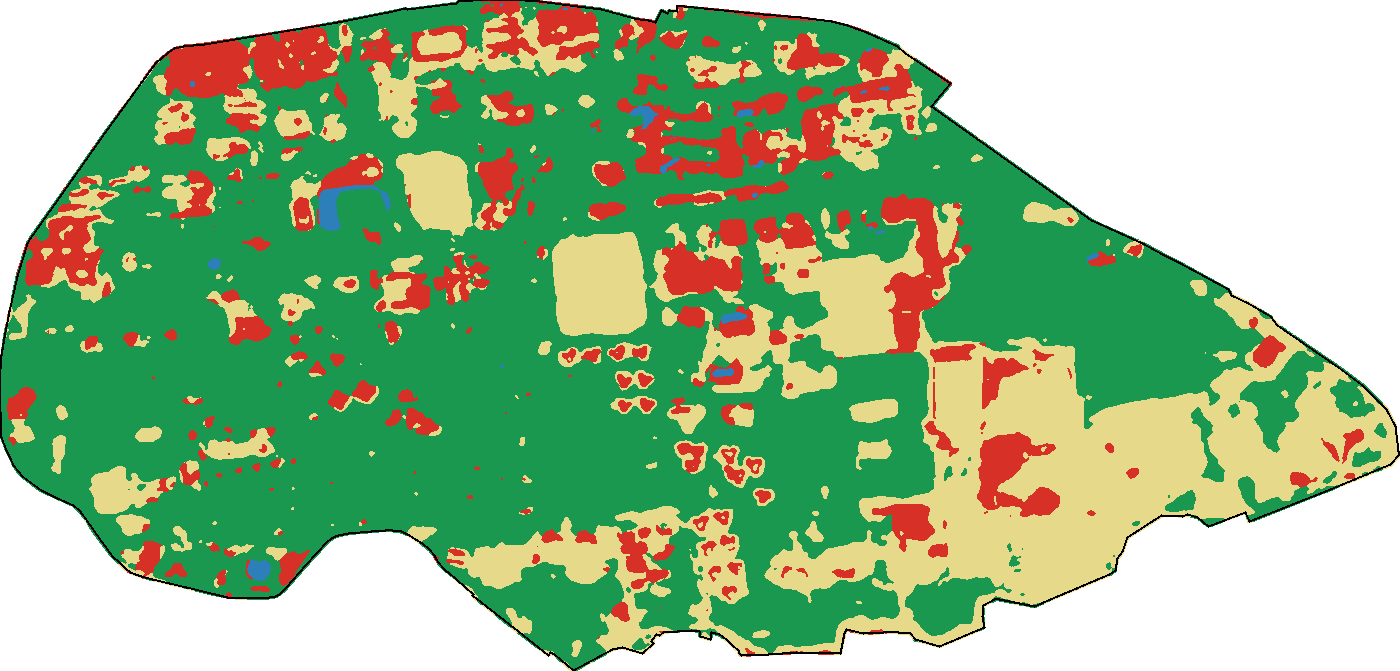
\includegraphics[width=10.6cm]{img/lulc_2025.png}};
  \node[anchor=north] at (tmap.south) {\small\classlegend};
  \node[anchor=south,text=muted,font=\scriptsize] at ([yshift=1mm]tmap.north) {2025 land cover map, Random Forest, 10 m};
\end{tikzpicture}
\end{frame}}

% ---------------------------------------------------------------- question
\begin{frame}{Can we measure how our own campus changed?}{BACKGROUND AND OBJECTIVES}
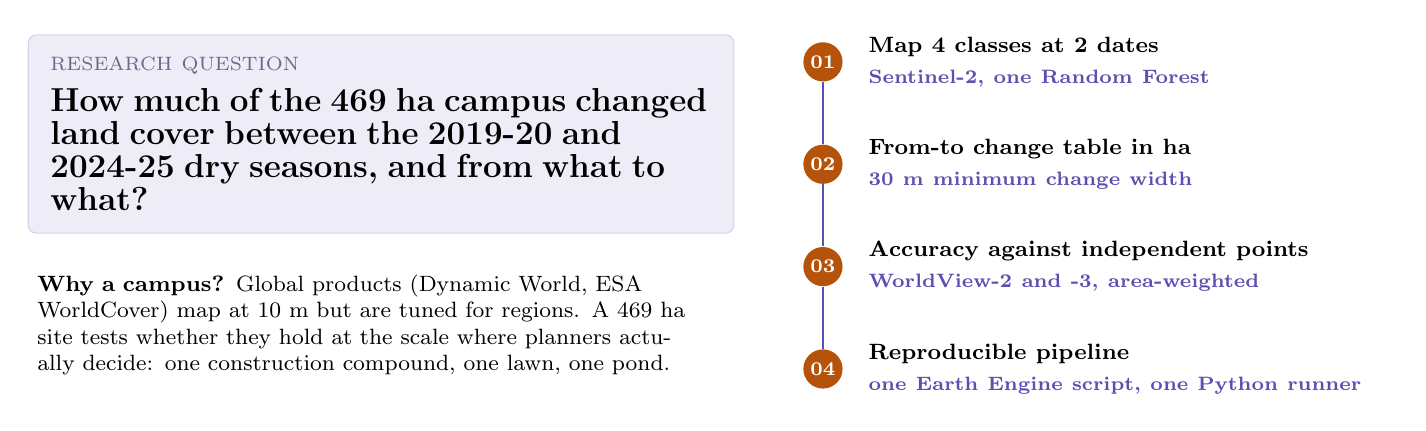
\begin{tikzpicture}
  \node[card,text width=8.4cm,inner sep=8pt,anchor=north west] (q) at (0,0) {%
    {\color{muted}\scriptsize RESEARCH QUESTION}\\[1mm]
    {\large\bfseries How much of the 469 ha campus changed land cover between the 2019-20 and 2024-25 dry seasons, and from what to what?}};
  \node[anchor=north west,text width=8.4cm,font=\footnotesize,below=4mm of q.south west,anchor=north west] (why) {%
    \textbf{Why a campus?} Global products (Dynamic World, ESA WorldCover) map at 10 m but are tuned for regions. A 469 ha site tests whether they hold at the scale where planners actually decide: one construction compound, one lawn, one pond.};
  \foreach \i/\t/\s in {1/Map 4 classes at 2 dates/Sentinel-2{,} one Random Forest,2/From-to change table in ha/30 m minimum change width,3/Accuracy against independent points/WorldView-2 and -3{,} area-weighted,4/Reproducible pipeline/one Earth Engine script{,} one Python runner}{
    \node[num] (n\i) at (10.1,-.35-1.3*\i+1.3) {0\i};
    \node[anchor=west,text width=6.6cm,align=left] at ($(n\i.east)+(.2,0)$) {\footnotesize\bfseries\t\\[-.3mm]\capt{\s}};
  }
  \draw[iris,line width=.8pt] (n1) -- (n2) -- (n3) -- (n4);
\end{tikzpicture}
\vfill

\begin{tikzpicture}
  \node[fill=ink,text=white,rounded corners=3pt,text width=17.2cm,inner sep=6pt,font=\scriptsize] {%
    \textbf{\color{gold}New in this version:} yearly dating of the south-east compound \textperiodcentered\ GLCM texture test \textperiodcentered\ is the change real? error-adjusted significance test \textperiodcentered\ change flow diagram \textperiodcentered\ gross gain, loss and swap per class \textperiodcentered\ map area vs point-based area with 95\% CI \textperiodcentered\ model tuning log with a held-out half \textperiodcentered\ feature importance \textperiodcentered\ WorldView validation design};
\end{tikzpicture}
\end{frame}

% ---------------------------------------------------------------- study area
\begin{frame}{A 469 ha fenced campus, mapped at 10 m}{STUDY AREA}
\begin{columns}[T]
\begin{column}{.6\textwidth}
  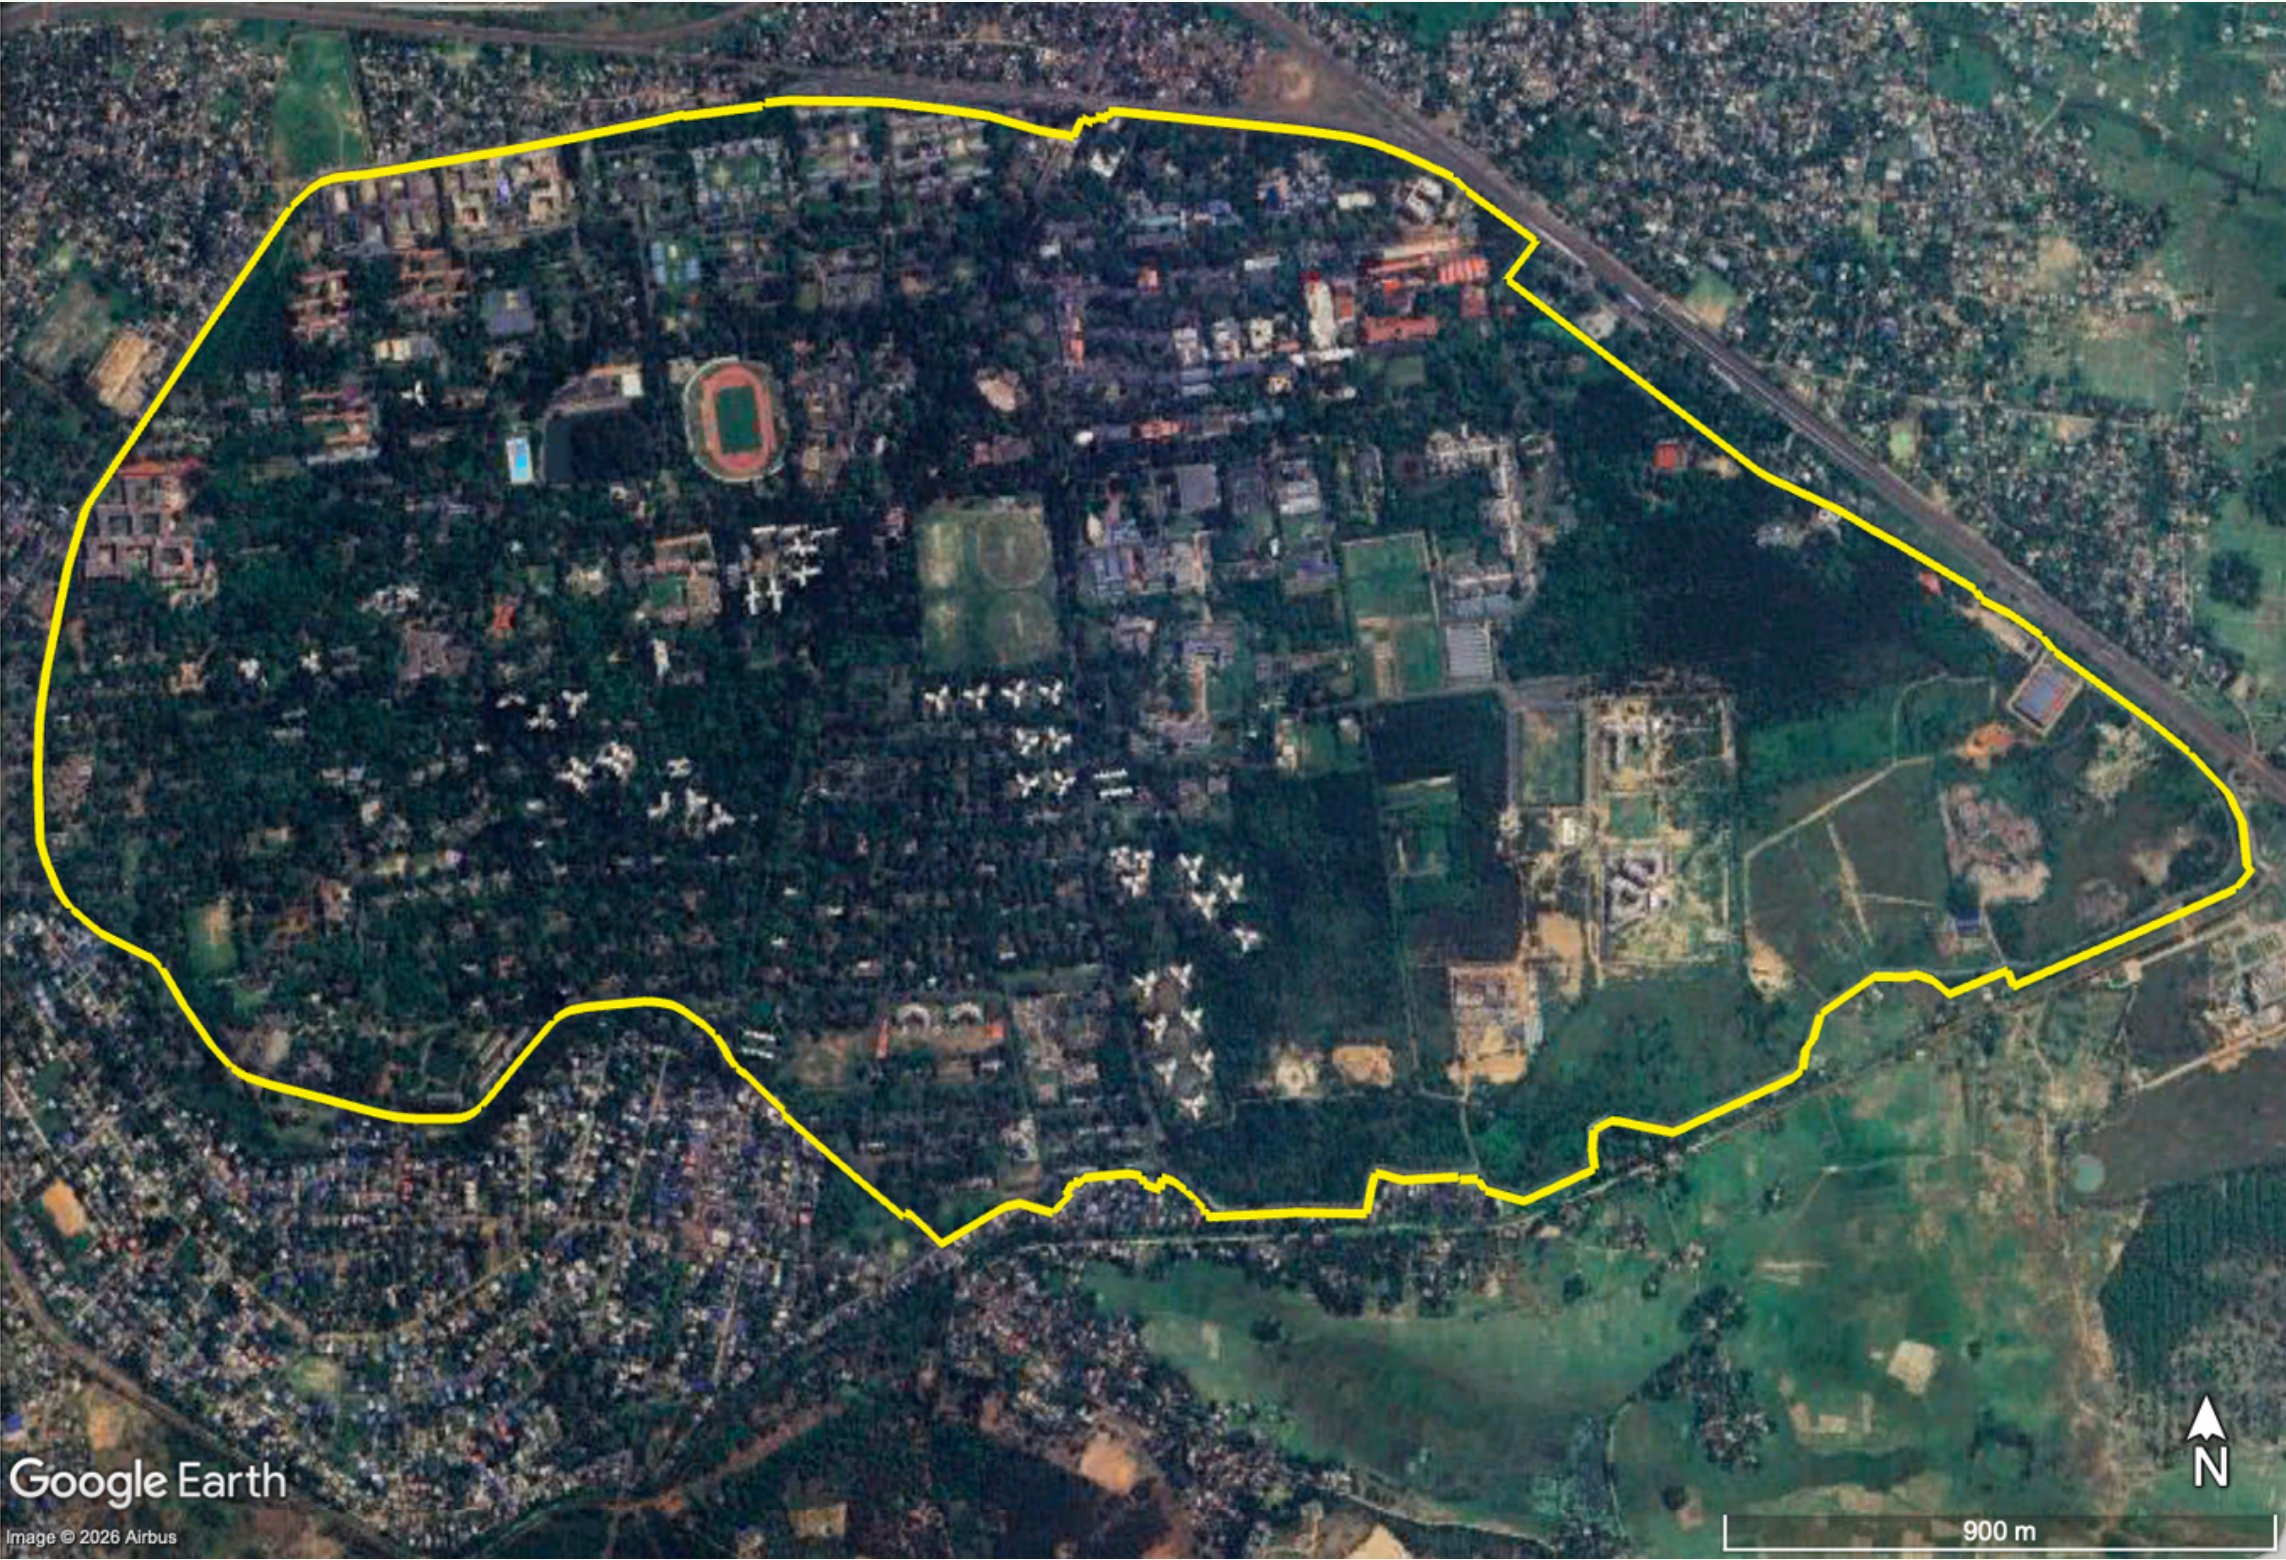
\includegraphics[width=\linewidth]{img/study_area-04.png}\\[-.5mm]
  \capt{Campus boundary: OpenStreetMap way 52435606 (184 vertices). Imagery: Google Earth, Airbus.}
\end{column}
\begin{column}{.36\textwidth}
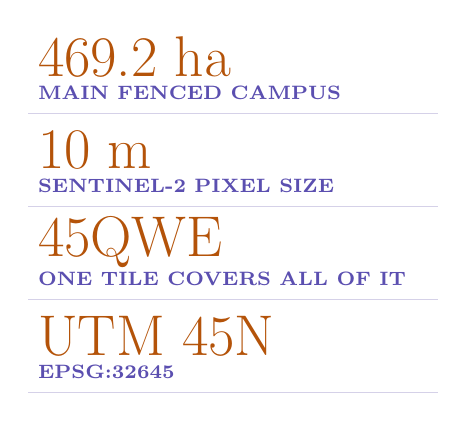
\begin{tikzpicture}
  \foreach \v/\l [count=\i] in {469.2 ha/MAIN FENCED CAMPUS,10 m/SENTINEL-2 PIXEL SIZE,45QWE/ONE TILE COVERS ALL OF IT,UTM 45N/EPSG:32645}{
    \node[anchor=west] at (0,-1.18*\i) {\bignum{\v}};
    \node[anchor=west] at (0,-1.18*\i-.46) {\capt{\l}};
    \draw[rule] (0,-1.18*\i-.72) -- (5.2,-1.18*\i-.72);
  }
\end{tikzpicture}\\[2mm]
{\scriptsize Halls and quarters outside the fence are not in the study area.}
\end{column}
\end{columns}
\end{frame}

% ---------------------------------------------------------------- pipeline
\begin{frame}{From 51 satellite scenes to a from-to change table}{METHOD \textperiodcentered\ END-TO-END PIPELINE}
\centering
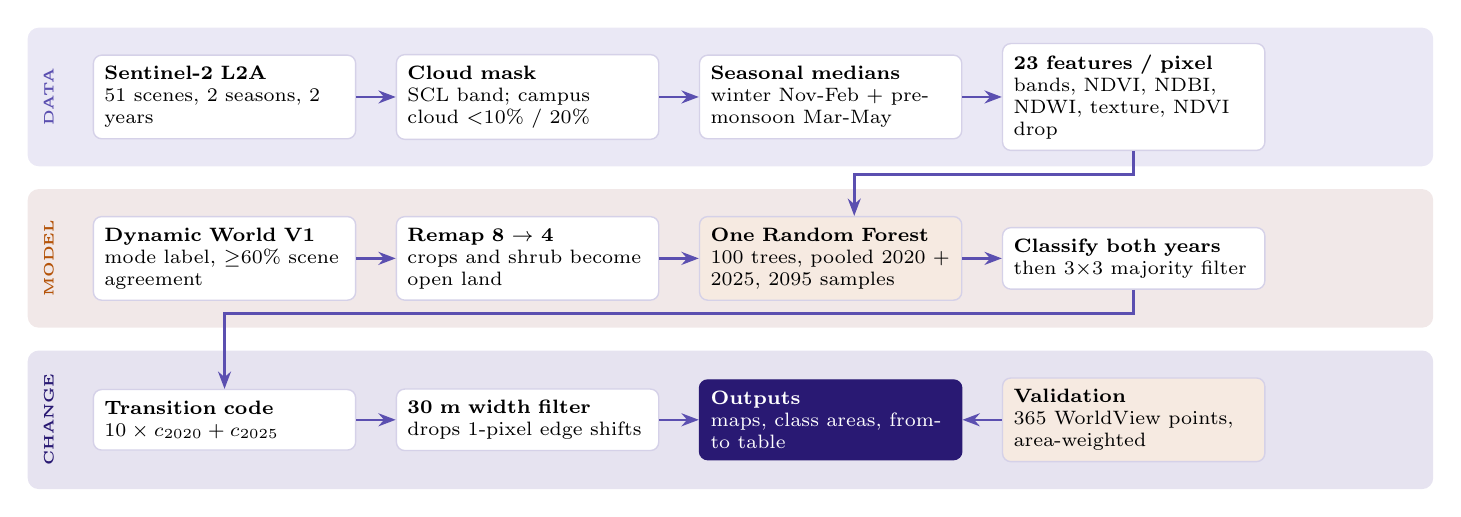
\begin{tikzpicture}[node distance=5mm,step/.append style={text width=3.05cm}]
  \foreach \y/\c/\t in {0/iris/DATA,-2.05/saffron/MODEL,-4.1/ink/CHANGE}{
    \fill[\c!8!bg,rounded corners=4pt] (-1.25,\y+.88) rectangle (16.6,\y-.88);
    \node[rotate=90,font=\tiny\bfseries,text=\c] at (-.98,\y) {\t};
  }
  \node[step] (s1) at (1.25,0) {\textbf{Sentinel-2 L2A}\\51 scenes, 2 seasons, 2 years};
  \node[step,right=of s1] (s2) {\textbf{Cloud mask}\\SCL band; campus cloud $<$10\% / 20\%};
  \node[step,right=of s2] (s3) {\textbf{Seasonal medians}\\winter Nov-Feb + pre-monsoon Mar-May};
  \node[step,right=of s3] (s4) {\textbf{23 features / pixel}\\bands, NDVI, NDBI, NDWI, texture, NDVI drop};
  \node[step] (m1) at (1.25,-2.05) {\textbf{Dynamic World V1}\\mode label, $\ge$60\% scene agreement};
  \node[step,right=of m1] (m2) {\textbf{Remap 8 \ra{} 4}\\crops and shrub become open land};
  \node[step,right=of m2,fill=saffron!12] (m3) {\textbf{One Random Forest}\\100 trees, pooled 2020 + 2025, 2095 samples};
  \node[step,right=of m3] (m4) {\textbf{Classify both years}\\then 3$\times$3 majority filter};
  \node[step] (c1) at (1.25,-4.1) {\textbf{Transition code}\\$10\times c_{2020} + c_{2025}$};
  \node[step,right=of c1] (c2) {\textbf{30 m width filter}\\drops 1-pixel edge shifts};
  \node[step,right=of c2,fill=ink,text=white,draw=ink] (c3) {\textbf{Outputs}\\maps, class areas, from-to table};
  \node[step,right=of c3,fill=saffron!12] (v1) {\textbf{Validation}\\365 WorldView points, area-weighted};
  \foreach \a/\b in {s1/s2,s2/s3,s3/s4,m1/m2,m2/m3,m3/m4,c1/c2,c2/c3}{\draw[flowarrow] (\a) -- (\b);}
  \draw[flowarrow] (v1) -- (c3);
  \draw[flowarrow] (s4.south) -- ++(0,-.3) -| ($(m3.north)+(.3,0)$);
  \draw[flowarrow] (m4.south) -- ++(0,-.3) -| (c1.north);
\end{tikzpicture}\\[3mm]

\begin{tikzpicture}
  \node[fill=ink,text=white,rounded corners=3pt,text width=17cm,inner sep=5pt,font=\scriptsize,align=center] {%
    One forest for both years, so an unchanged pixel gets the same rules in 2020 and 2025. Separate forests disagreed on 91 ha of unchanged roofs.};
\end{tikzpicture}
\end{frame}

% ---------------------------------------------------------------- data
\begin{frame}{Same seasons in both years, so seasonal greening is not counted as change}{DATA}
\begin{columns}[T]
\begin{column}{.49\textwidth}\centering
  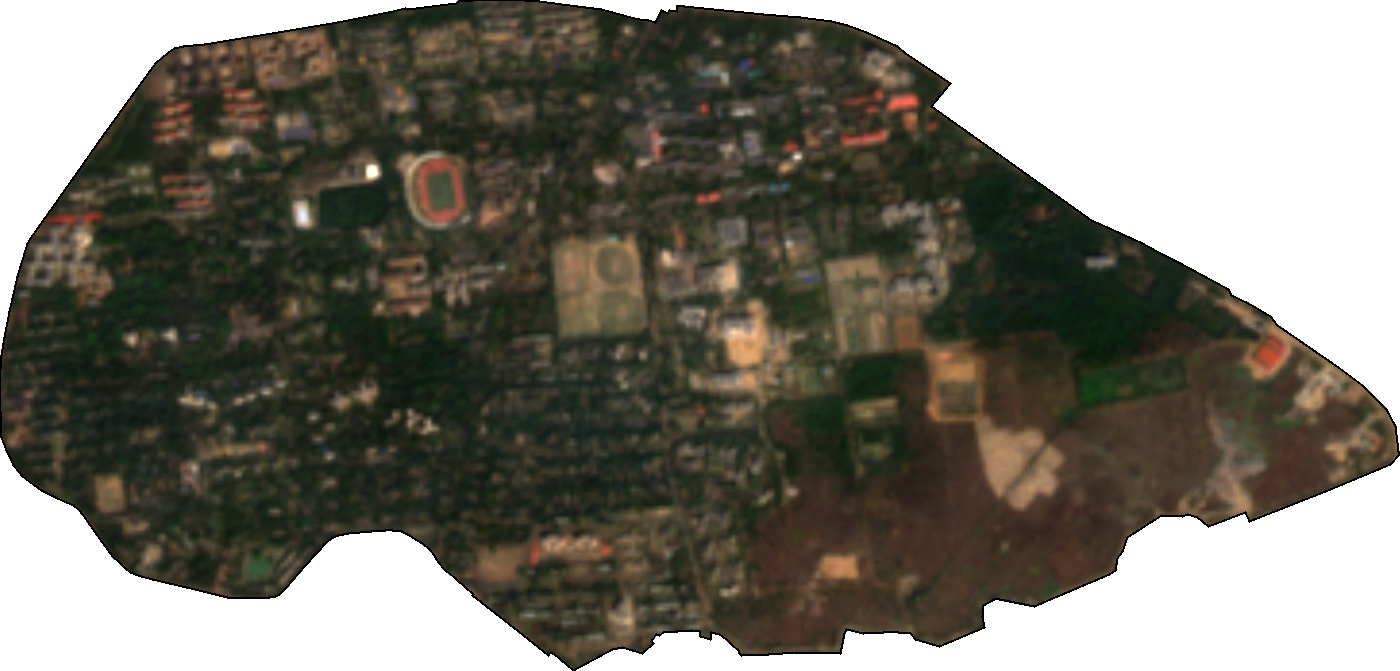
\includegraphics[width=\linewidth]{img/true_colour_2020.png}\\\capt{Winter 2019-20 median composite, 11 scenes}
\end{column}
\begin{column}{.49\textwidth}\centering
  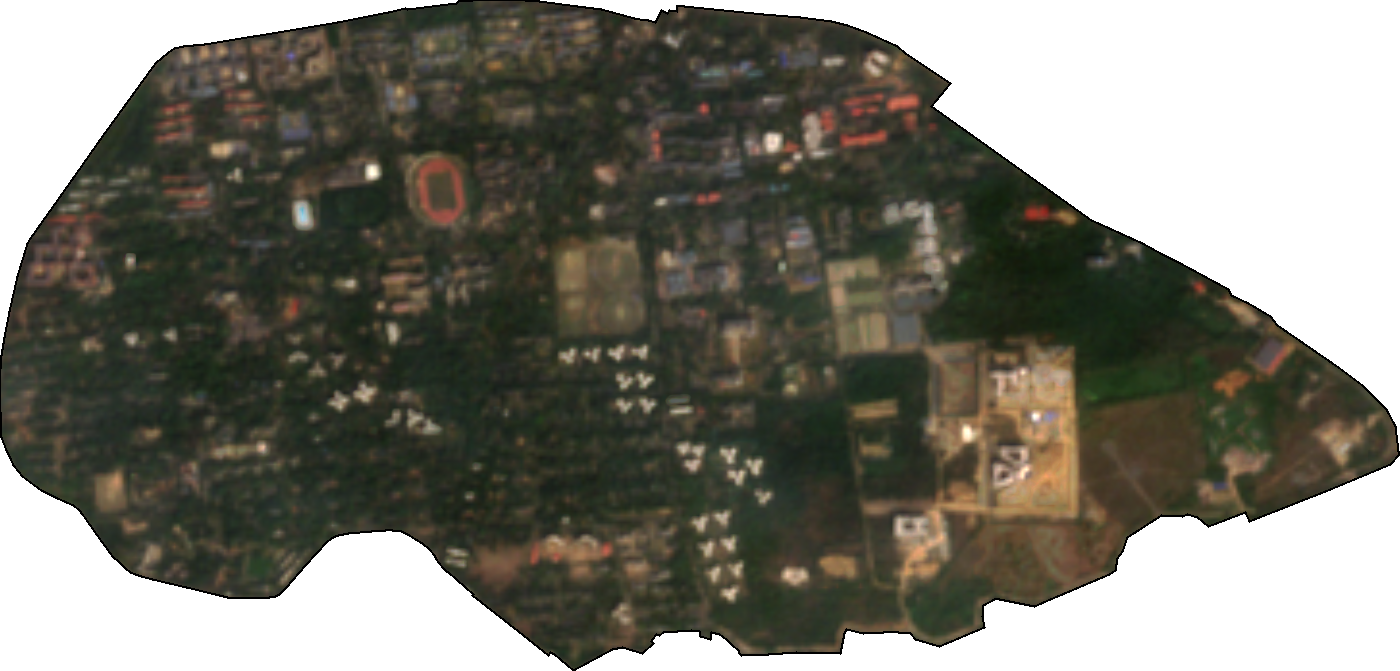
\includegraphics[width=\linewidth]{img/true_colour_2025.png}\\\capt{Winter 2024-25 median composite, 16 scenes}
\end{column}
\end{columns}
\vspace{3mm}
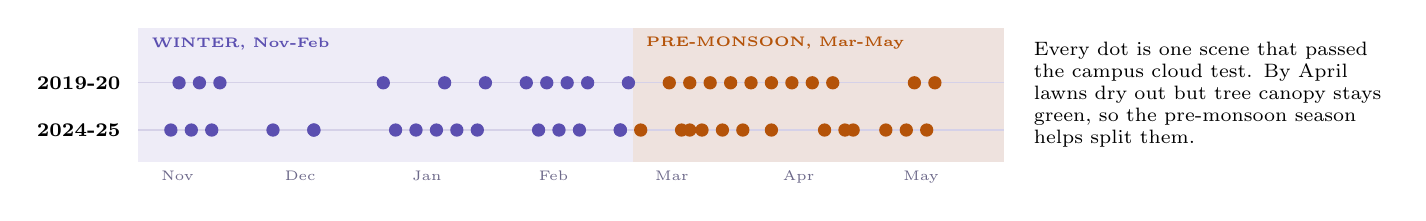
\begin{tikzpicture}
  \begin{scope}[xshift=1.5cm]\fill[haze] (0,-0.25) rectangle (6.278,1.45); \fill[saffron!12!bg] (6.278,-0.25) rectangle (11.0,1.45);
\node[font=\tiny\bfseries,text=iris,anchor=north west] at (0.05,1.45) {WINTER, Nov-Feb};
\node[font=\tiny\bfseries,text=saffron,anchor=north west] at (6.328,1.45) {PRE-MONSOON, Mar-May};
\node[anchor=east,font=\scriptsize\bfseries] at (-0.1,0.75) {2019-20};
\draw[rule] (0,0.75) -- (11.0,0.75);
\fill[iris] (0.519,0.75) circle (2.4pt);
\fill[iris] (0.778,0.75) circle (2.4pt);
\fill[iris] (1.038,0.75) circle (2.4pt);
\fill[iris] (3.113,0.75) circle (2.4pt);
\fill[iris] (3.892,0.75) circle (2.4pt);
\fill[iris] (4.410,0.75) circle (2.4pt);
\fill[iris] (4.929,0.75) circle (2.4pt);
\fill[iris] (5.189,0.75) circle (2.4pt);
\fill[iris] (5.448,0.75) circle (2.4pt);
\fill[iris] (5.708,0.75) circle (2.4pt);
\fill[iris] (6.226,0.75) circle (2.4pt);
\fill[saffron] (6.745,0.75) circle (2.4pt);
\fill[saffron] (7.005,0.75) circle (2.4pt);
\fill[saffron] (7.264,0.75) circle (2.4pt);
\fill[saffron] (7.524,0.75) circle (2.4pt);
\fill[saffron] (7.783,0.75) circle (2.4pt);
\fill[saffron] (8.042,0.75) circle (2.4pt);
\fill[saffron] (8.302,0.75) circle (2.4pt);
\fill[saffron] (8.561,0.75) circle (2.4pt);
\fill[saffron] (8.821,0.75) circle (2.4pt);
\fill[saffron] (9.858,0.75) circle (2.4pt);
\fill[saffron] (10.118,0.75) circle (2.4pt);
\node[anchor=east,font=\scriptsize\bfseries] at (-0.1,0.15000000000000002) {2024-25};
\draw[rule] (0,0.15000000000000002) -- (11.0,0.15000000000000002);
\fill[iris] (0.415,0.15000000000000002) circle (2.4pt);
\fill[iris] (0.675,0.15000000000000002) circle (2.4pt);
\fill[iris] (0.934,0.15000000000000002) circle (2.4pt);
\fill[iris] (1.712,0.15000000000000002) circle (2.4pt);
\fill[iris] (2.231,0.15000000000000002) circle (2.4pt);
\fill[iris] (2.231,0.15000000000000002) circle (2.4pt);
\fill[iris] (3.269,0.15000000000000002) circle (2.4pt);
\fill[iris] (3.528,0.15000000000000002) circle (2.4pt);
\fill[iris] (3.788,0.15000000000000002) circle (2.4pt);
\fill[iris] (4.047,0.15000000000000002) circle (2.4pt);
\fill[iris] (4.307,0.15000000000000002) circle (2.4pt);
\fill[iris] (5.085,0.15000000000000002) circle (2.4pt);
\fill[iris] (5.344,0.15000000000000002) circle (2.4pt);
\fill[iris] (5.604,0.15000000000000002) circle (2.4pt);
\fill[iris] (6.123,0.15000000000000002) circle (2.4pt);
\fill[iris] (6.123,0.15000000000000002) circle (2.4pt);
\fill[saffron] (6.382,0.15000000000000002) circle (2.4pt);
\fill[saffron] (6.901,0.15000000000000002) circle (2.4pt);
\fill[saffron] (7.005,0.15000000000000002) circle (2.4pt);
\fill[saffron] (7.160,0.15000000000000002) circle (2.4pt);
\fill[saffron] (7.420,0.15000000000000002) circle (2.4pt);
\fill[saffron] (7.679,0.15000000000000002) circle (2.4pt);
\fill[saffron] (8.042,0.15000000000000002) circle (2.4pt);
\fill[saffron] (8.717,0.15000000000000002) circle (2.4pt);
\fill[saffron] (8.976,0.15000000000000002) circle (2.4pt);
\fill[saffron] (9.080,0.15000000000000002) circle (2.4pt);
\fill[saffron] (9.495,0.15000000000000002) circle (2.4pt);
\fill[saffron] (9.755,0.15000000000000002) circle (2.4pt);
\fill[saffron] (10.014,0.15000000000000002) circle (2.4pt);
\node[font=\tiny,text=muted,anchor=north] at (0.500,-0.25) {Nov};
\node[font=\tiny,text=muted,anchor=north] at (2.057,-0.25) {Dec};
\node[font=\tiny,text=muted,anchor=north] at (3.665,-0.25) {Jan};
\node[font=\tiny,text=muted,anchor=north] at (5.274,-0.25) {Feb};
\node[font=\tiny,text=muted,anchor=north] at (6.778,-0.25) {Mar};
\node[font=\tiny,text=muted,anchor=north] at (8.387,-0.25) {Apr};
\node[font=\tiny,text=muted,anchor=north] at (9.943,-0.25) {May};
\end{scope}
  \node[anchor=west,text width=4.5cm,font=\scriptsize] at (12.75,.6) {Every dot is one scene that passed the campus cloud test. By April lawns dry out but tree canopy stays green, so the pre-monsoon season helps split them.};
\end{tikzpicture}
\end{frame}

% ---------------------------------------------------------------- classes
\begin{frame}{Eight Dynamic World labels collapse into four campus classes}{CLASSES}
\begin{columns}[c]
\begin{column}{.5\textwidth}
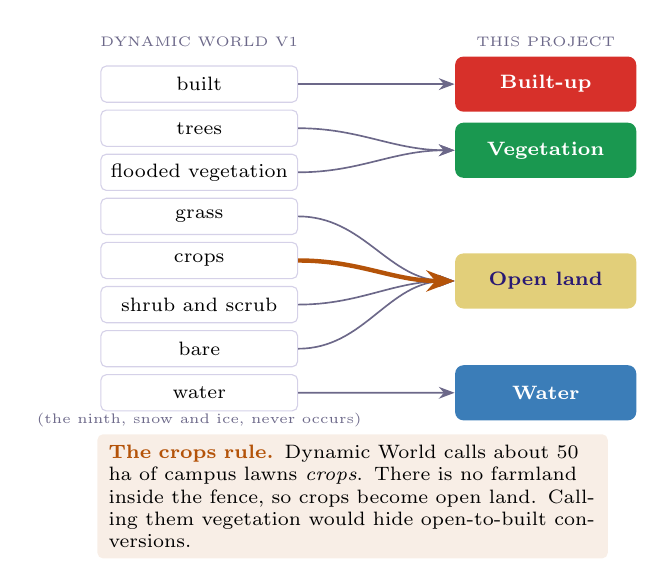
\begin{tikzpicture}[lab/.style={font=\scriptsize,fill=white,draw=rule,rounded corners=2pt,minimum width=2.5cm,minimum height=4.6mm},
  cls/.style={font=\scriptsize\bfseries,rounded corners=3pt,minimum width=2.3cm,minimum height=7mm,text=white}]
  \foreach \t [count=\i] in {built,trees,flooded vegetation,grass,crops,shrub and scrub,bare,water}{\node[lab] (d\i) at (0,-.56*\i) {\t};}
  \node[cls,fill=cbuilt] (B) at (4.4,-.56) {Built-up};
  \node[cls,fill=cveg] (V) at (4.4,-1.4) {Vegetation};
  \node[cls,fill=copen,text=ink] (O) at (4.4,-3.06) {Open land};
  \node[cls,fill=cwater] (W) at (4.4,-4.48) {Water};
  \foreach \i/\c in {1/B,2/V,3/V,4/O,6/O,7/O,8/W}{\draw[-{Stealth},muted,line width=.6pt] (d\i.east) to[out=0,in=180] (\c.west);}
  \draw[-{Stealth},saffron,line width=1.6pt] (d5.east) to[out=0,in=180] (O.west);
  \node[font=\tiny,text=muted] at (0,-.02) {DYNAMIC WORLD V1};
  \node[font=\tiny,text=muted] at (0,-4.83) {(the ninth, snow and ice, never occurs)};
  \node[font=\tiny,text=muted] at (4.4,-.02) {THIS PROJECT};
  \node[text width=6.2cm,font=\scriptsize,anchor=north west,fill=saffron!10,rounded corners=2pt,inner sep=4pt] at (-1.3,-5.0) {\textbf{\color{saffron}The crops rule.} Dynamic World calls about 50 ha of campus lawns \emph{crops}. There is no farmland inside the fence, so crops become open land. Calling them vegetation would hide open-to-built conversions.};
\end{tikzpicture}
\end{column}
\begin{column}{.46\textwidth}
\begin{tikzpicture}
  \foreach \i/\n/\c/\d in {0/Built-up/cbuilt/roofs{,} roads{,} courts,1/Vegetation/cveg/canopy{,} dense woody,2/Open land/copen/lawns{,} fields{,} bare plots,3/Water/cwater/ponds{,} tanks}{
    \pgfmathsetmacro\x{mod(\i,2)*3.4}
    \pgfmathsetmacro\y{-int(\i/2)*3.6}
    \node[anchor=north west,inner sep=0] (im\i) at (\x,\y) {\includegraphics[width=2.75cm]{img/chip\i-07.png}};
    \fill[\c] (im\i.south west) rectangle ([yshift=-1.2mm]im\i.south east);
    \node[anchor=north west,font=\scriptsize\bfseries,inner sep=1pt] at ([yshift=-1.6mm]im\i.south west) {\n};
    \node[anchor=north west,font=\tiny,text=muted,inner sep=1pt] at ([yshift=-5.2mm]im\i.south west) {\d};
  }
\end{tikzpicture}
\end{column}
\end{columns}
\end{frame}

% ---------------------------------------------------------------- features
\begin{frame}{23 features per pixel; the seasonal and texture ones earn their place}{FEATURES AND FEATURE IMPORTANCE}
\begin{columns}[T]
\begin{column}{.47\textwidth}
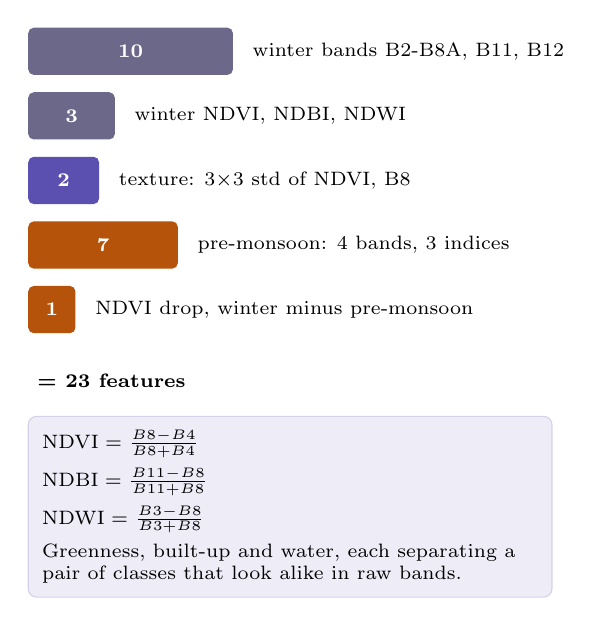
\begin{tikzpicture}
  \foreach \n/\w/\l/\c [count=\i] in {10/2.6/winter bands B2-B8A{,} B11{,} B12/muted,3/1.1/winter NDVI{,} NDBI{,} NDWI/muted,2/.9/texture: 3$\times$3 std of NDVI{,} B8/iris,7/1.9/pre-monsoon: 4 bands{,} 3 indices/saffron,1/.6/NDVI drop{,} winter minus pre-monsoon/saffron}{
    \node[fill=\c,text=white,font=\scriptsize\bfseries,minimum width=\w cm,minimum height=6mm,rounded corners=2pt,anchor=west] (b\i) at (0,-.82*\i) {\n};
    \node[anchor=west,font=\scriptsize] at ($(b\i.east)+(.12,0)$) {\l};
  }
  \node[anchor=west,font=\scriptsize\bfseries] at (0,-5.0) {= 23 features};
  \node[card,anchor=north west,text width=6.3cm,inner sep=5pt,font=\scriptsize] at (0,-5.45) {%
    $\mathrm{NDVI}=\frac{B8-B4}{B8+B4}$\\[1mm] $\mathrm{NDBI}=\frac{B11-B8}{B11+B8}$\\[1mm] $\mathrm{NDWI}=\frac{B3-B8}{B3+B8}$\\[1mm]
    Greenness, built-up and water, each separating a pair of classes that look alike in raw bands.};
\end{tikzpicture}
\end{column}
\begin{column}{.5\textwidth}
\capt{RANDOM FOREST IMPORTANCE, TOP 10 OF 23 (GINI, EARTH ENGINE)}\\[2mm]
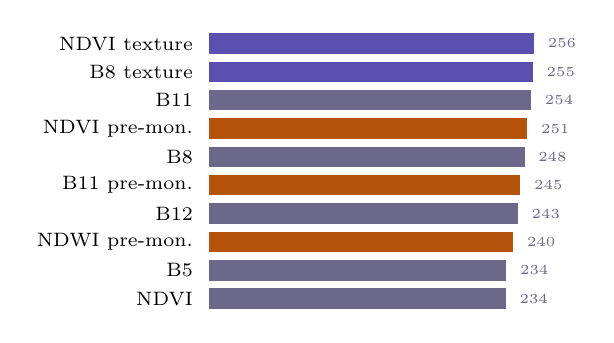
\begin{tikzpicture}\fill[iris] (0,-0.130) rectangle (4.130,0.130);
\node[anchor=east,font=\scriptsize] at (-0.08,0.000) {NDVI texture};
\node[anchor=west,font=\tiny,text=muted] at (4.180,0.000) {256};
\fill[iris] (0,-0.490) rectangle (4.115,-0.230);
\node[anchor=east,font=\scriptsize] at (-0.08,-0.360) {B8 texture};
\node[anchor=west,font=\tiny,text=muted] at (4.165,-0.360) {255};
\fill[muted] (0,-0.850) rectangle (4.093,-0.590);
\node[anchor=east,font=\scriptsize] at (-0.08,-0.720) {B11};
\node[anchor=west,font=\tiny,text=muted] at (4.143,-0.720) {254};
\fill[saffron] (0,-1.210) rectangle (4.044,-0.950);
\node[anchor=east,font=\scriptsize] at (-0.08,-1.080) {NDVI pre-mon.};
\node[anchor=west,font=\tiny,text=muted] at (4.094,-1.080) {251};
\fill[muted] (0,-1.570) rectangle (4.008,-1.310);
\node[anchor=east,font=\scriptsize] at (-0.08,-1.440) {B8};
\node[anchor=west,font=\tiny,text=muted] at (4.058,-1.440) {248};
\fill[saffron] (0,-1.930) rectangle (3.956,-1.670);
\node[anchor=east,font=\scriptsize] at (-0.08,-1.800) {B11 pre-mon.};
\node[anchor=west,font=\tiny,text=muted] at (4.006,-1.800) {245};
\fill[muted] (0,-2.290) rectangle (3.924,-2.030);
\node[anchor=east,font=\scriptsize] at (-0.08,-2.160) {B12};
\node[anchor=west,font=\tiny,text=muted] at (3.974,-2.160) {243};
\fill[saffron] (0,-2.650) rectangle (3.865,-2.390);
\node[anchor=east,font=\scriptsize] at (-0.08,-2.520) {NDWI pre-mon.};
\node[anchor=west,font=\tiny,text=muted] at (3.915,-2.520) {240};
\fill[muted] (0,-3.010) rectangle (3.777,-2.750);
\node[anchor=east,font=\scriptsize] at (-0.08,-2.880) {B5};
\node[anchor=west,font=\tiny,text=muted] at (3.827,-2.880) {234};
\fill[muted] (0,-3.370) rectangle (3.771,-3.110);
\node[anchor=east,font=\scriptsize] at (-0.08,-3.240) {NDVI};
\node[anchor=west,font=\tiny,text=muted] at (3.821,-3.240) {234};
\end{tikzpicture}\\[2mm]
{\scriptsize\sw{saffron} pre-monsoon \quad \sw{iris} texture \quad \sw{muted} winter}\\[2mm]
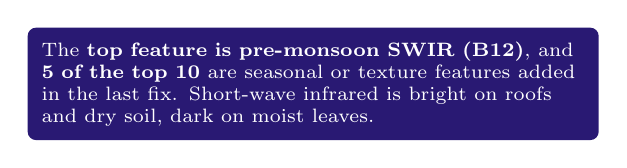
\begin{tikzpicture}
  \node[fill=ink,text=white,rounded corners=3pt,text width=6.9cm,inner sep=5pt,font=\scriptsize] {The \textbf{top feature is pre-monsoon SWIR (B12)}, and \textbf{5 of the top 10} are seasonal or texture features added in the last fix. Short-wave infrared is bright on roofs and dry soil, dark on moist leaves.};
\end{tikzpicture}
\end{column}
\end{columns}
\end{frame}

% ---------------------------------------------------------------- tuning
\begin{frame}{Tuning the model: three runs, each fix aimed at one measured error}{MODEL TUNING LOG}
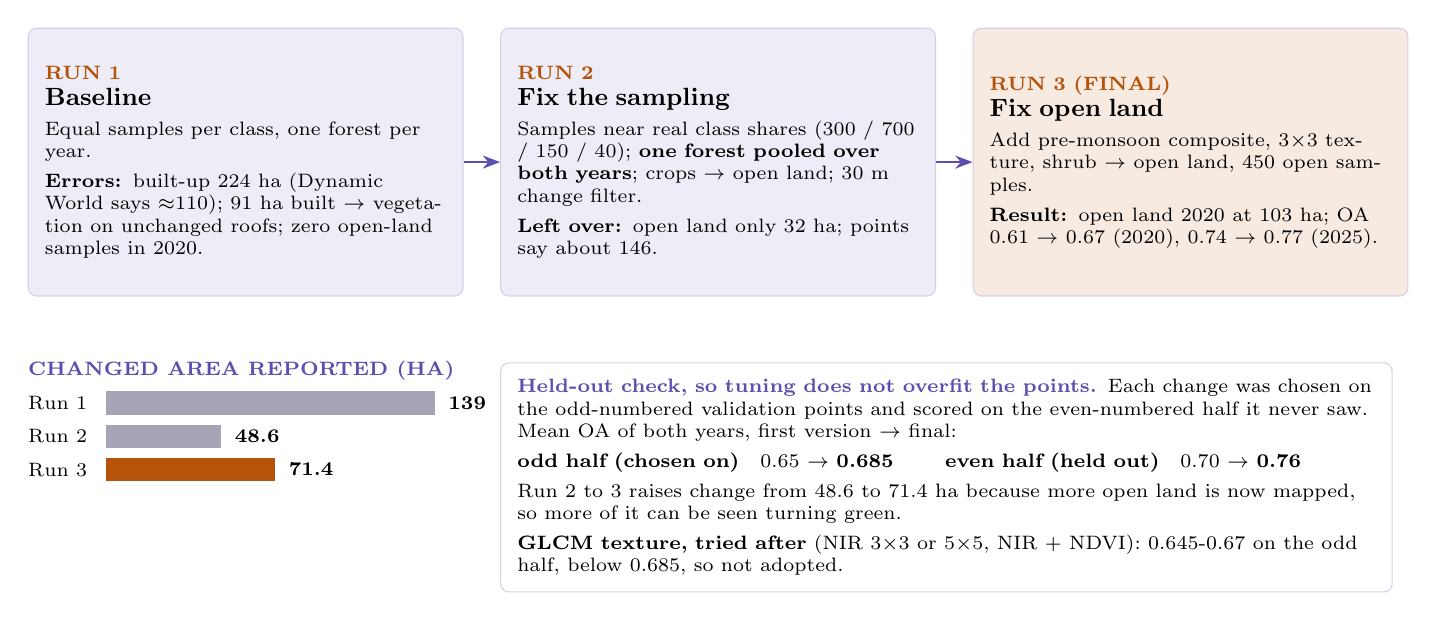
\begin{tikzpicture}[run/.style={card,text width=5.1cm,inner sep=6pt,font=\scriptsize,anchor=north west,minimum height=3.4cm}]
  \node[run] (r1) at (0,0) {%
    {\color{saffron}\bfseries RUN 1}\\[.5mm]{\small\bfseries Baseline}\\[1mm]
    Equal samples per class, one forest per year.\\[1mm]
    \textbf{Errors:} built-up 224 ha (Dynamic World says $\approx$110); 91 ha built \ra{} vegetation on unchanged roofs; zero open-land samples in 2020.};
  \node[run] (r2) at (6.0,0) {%
    {\color{saffron}\bfseries RUN 2}\\[.5mm]{\small\bfseries Fix the sampling}\\[1mm]
    Samples near real class shares (300 / 700 / 150 / 40); \textbf{one forest pooled over both years}; crops \ra{} open land; 30 m change filter.\\[1mm]
    \textbf{Left over:} open land only 32 ha; points say about 146.};
  \node[run,fill=saffron!12] (r3) at (12.0,0) {%
    {\color{saffron}\bfseries RUN 3 (FINAL)}\\[.5mm]{\small\bfseries Fix open land}\\[1mm]
    Add pre-monsoon composite, 3$\times$3 texture, shrub \ra{} open land, 450 open samples.\\[1mm]
    \textbf{Result:} open land 2020 at 103 ha; OA 0.61 \ra{} 0.67 (2020), 0.74 \ra{} 0.77 (2025).};
  \draw[flowarrow] (r1.east) -- (r2.west);
  \draw[flowarrow] (r2.east) -- (r3.west);
  % changed area bars
  \begin{scope}[yshift=-4.5cm]
    \node[anchor=west,inner sep=0] at (0,.15) {\capt{CHANGED AREA REPORTED (HA)}};
    \foreach \v/\l/\c [count=\i] in {139/Run 1/muted!60,48.6/Run 2/muted!60,71.4/Run 3/saffron}{
      \fill[\c] (1.0,-.42*\i) rectangle (1.0+\v*.03,-.42*\i+.3);
      \node[anchor=west,font=\scriptsize,inner sep=0] at (0,-.42*\i+.15) {\l};
      \node[anchor=west,font=\scriptsize\bfseries] at (1.0+\v*.03+.05,-.42*\i+.15) {\v};
    }
  \end{scope}
  \node[anchor=north west,text width=10.9cm,font=\scriptsize,fill=white,draw=rule,rounded corners=3pt,inner sep=6pt] at (6.0,-4.25) {%
    {\color{iris}\bfseries Held-out check, so tuning does not overfit the points.} Each change was chosen on the odd-numbered validation points and scored on the even-numbered half it never saw. Mean OA of both years, first version \ra{} final:\\[1mm]
    \textbf{odd half (chosen on)} \; 0.65 \ra{} \textbf{0.685} \qquad \textbf{even half (held out)} \; 0.70 \ra{} \textbf{0.76}\\[1mm]
    Run 2 to 3 raises change from 48.6 to 71.4 ha because more open land is now mapped, so more of it can be seen turning green.\\[1mm]
    \textbf{GLCM texture, tried after} (NIR 3$\times$3 or 5$\times$5, NIR + NDVI): 0.645-0.67 on the odd half, below 0.685, so not adopted.};
\end{tikzpicture}
\end{frame}

% ---------------------------------------------------------------- maps and change
\begin{frame}{Vegetation grew, open land shrank: 15.2\% of the campus changed}{RESULT \textperiodcentered\ LAND COVER MAPS AND CHANGE}
\begin{columns}[T]
\begin{column}{.4\textwidth}
% labels sit in the empty north-west corner of each map's bounding box
\begin{tikzpicture}
  \node[inner sep=0,anchor=north west] (m20) at (0,0) {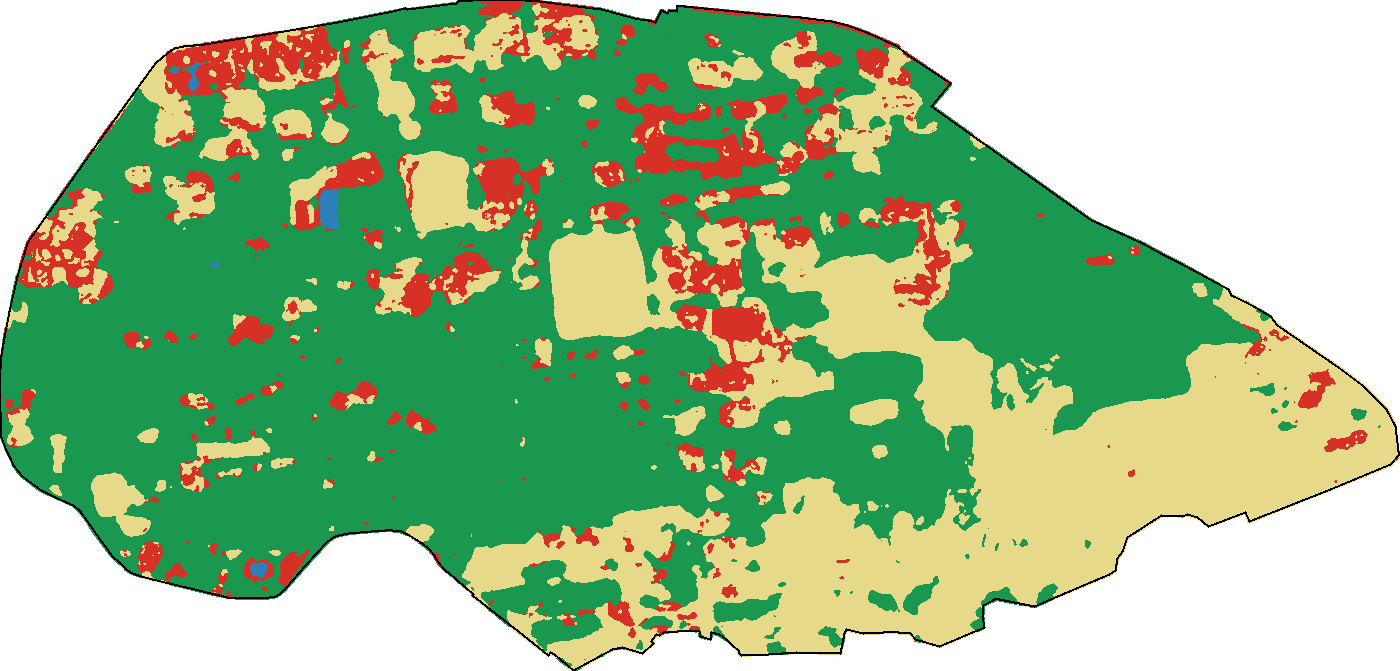
\includegraphics[width=\linewidth]{img/lulc_2020.png}};
  \node[inner sep=0,anchor=north west] (m25) at ([yshift=-2mm]m20.south west) {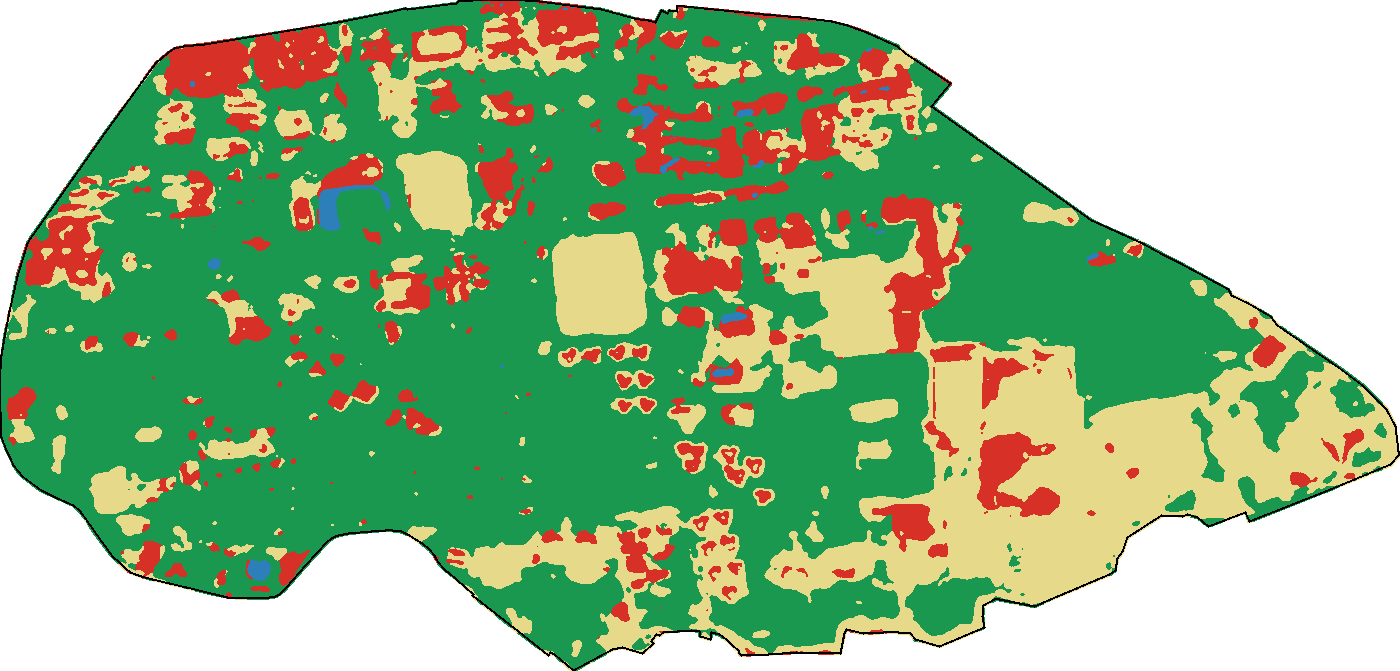
\includegraphics[width=\linewidth]{img/lulc_2025.png}};
  \node[inner sep=0,anchor=north west] at (m20.north west) {\capt{2020}};
  \node[inner sep=0,anchor=north west] at (m25.north west) {\capt{2025}};
\end{tikzpicture}\\[1.5mm]
  {\scriptsize\classlegend}
\end{column}
\begin{column}{.57\textwidth}\centering
\begin{tikzpicture}
  \node[inner sep=0] (chg) {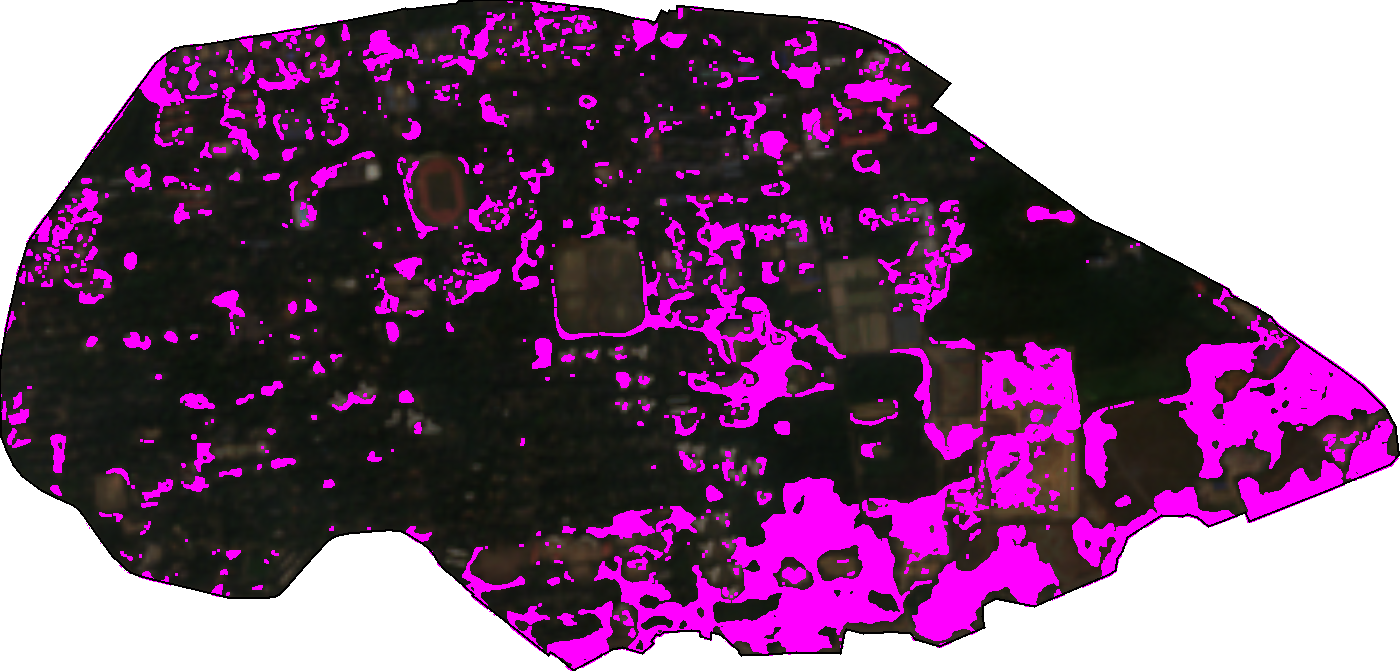
\includegraphics[width=.94\linewidth]{img/change_2020_2025.png}};
  \node[inner sep=0,anchor=north east] at (chg.north east) {\capt{CHANGE 2020 \ra{} 2025}};
\end{tikzpicture}\\[.3mm]
  {\scriptsize\color{muted}Magenta: changed patches at least 30 m wide, over the 2025 image}\\[3mm]
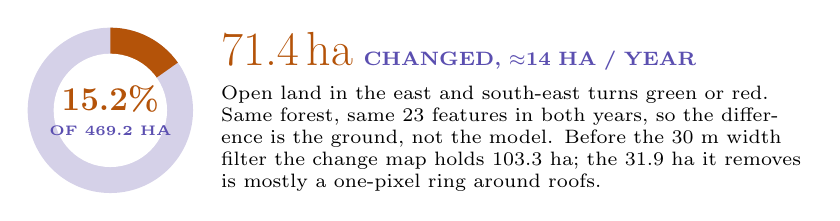
\begin{tikzpicture}
  \fill[rule] (0,0) circle (1.05);
  \fill[saffron] (0,0) -- (90:1.05) arc[start angle=90,end angle={90-0.152*360},radius=1.05] -- cycle;
  \fill[white] (0,0) circle (.72);
  \node[align=center] at (0,0) {{\color{saffron}\fontsize{12}{13}\selectfont\bfseries 15.2\%}\\[-1mm]{\color{iris}\fontsize{5}{6}\selectfont\bfseries OF 469.2 HA}};
  \node[anchor=north west,text width=7.5cm,font=\scriptsize,align=left,inner sep=0] at (1.4,1.0) {%
    {\color{saffron}\fontsize{16}{18}\selectfont 71.4 ha}\enspace\capt{CHANGED, $\approx$14 HA / YEAR}\\[1.5mm]
    Open land in the east and south-east turns green or red. Same forest, same 23 features in both years, so the difference is the ground, not the model. Before the 30 m width filter the change map holds 103.3 ha; the 31.9 ha it removes is mostly a one-pixel ring around roofs.};
\end{tikzpicture}
\end{column}
\end{columns}
\end{frame}

% ---------------------------------------------------------------- area
\begin{frame}{Vegetation +42.2 ha, open land $-$46.8 ha; the points agree on both}{RESULT \textperiodcentered\ AREA BY CLASS, TWO ESTIMATES}
\begin{columns}[c]
\begin{column}{.66\textwidth}
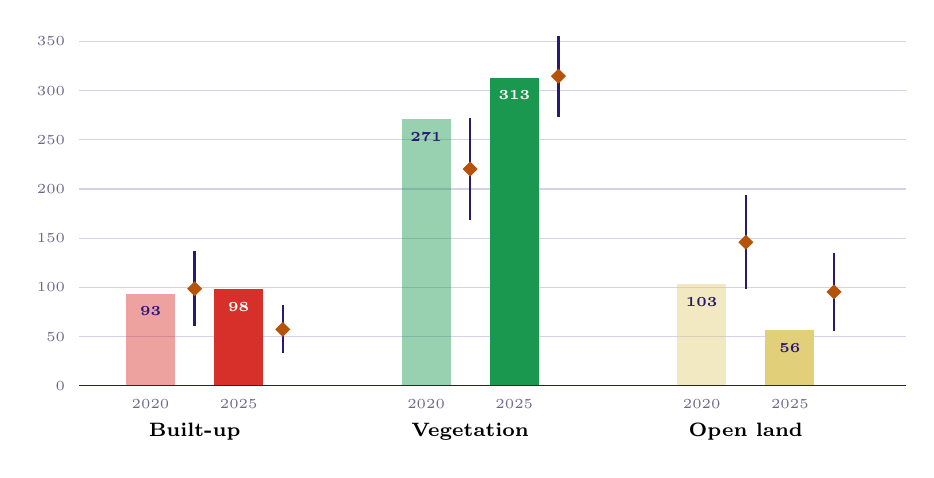
\begin{tikzpicture}\draw[rule] (-0.2,0.000) -- (10.3,0.000); \node[anchor=east,font=\tiny,text=muted] at (-0.25,0.000) {0};
\draw[rule] (-0.2,0.625) -- (10.3,0.625); \node[anchor=east,font=\tiny,text=muted] at (-0.25,0.625) {50};
\draw[rule] (-0.2,1.250) -- (10.3,1.250); \node[anchor=east,font=\tiny,text=muted] at (-0.25,1.250) {100};
\draw[rule] (-0.2,1.875) -- (10.3,1.875); \node[anchor=east,font=\tiny,text=muted] at (-0.25,1.875) {150};
\draw[rule] (-0.2,2.500) -- (10.3,2.500); \node[anchor=east,font=\tiny,text=muted] at (-0.25,2.500) {200};
\draw[rule] (-0.2,3.125) -- (10.3,3.125); \node[anchor=east,font=\tiny,text=muted] at (-0.25,3.125) {250};
\draw[rule] (-0.2,3.750) -- (10.3,3.750); \node[anchor=east,font=\tiny,text=muted] at (-0.25,3.750) {300};
\draw[rule] (-0.2,4.375) -- (10.3,4.375); \node[anchor=east,font=\tiny,text=muted] at (-0.25,4.375) {350};
\fill[cbuilt,fill opacity=0.45] (0.400,0) rectangle (1.020,1.168);
\node[font=\tiny\bfseries,text=ink,anchor=north] at (0.710,1.128) {93};
\draw[ink,line width=.9pt] (1.270,0.755) -- (1.270,1.710);
\node[diamond,fill=saffron,inner sep=1.4pt] at (1.270,1.232) {};
\node[font=\tiny,text=muted,anchor=north] at (0.710,-0.05) {2020};
\fill[cbuilt,fill opacity=1] (1.520,0) rectangle (2.140,1.225);
\node[font=\tiny\bfseries,text=white,anchor=north] at (1.830,1.185) {98};
\draw[ink,line width=.9pt] (2.390,0.413) -- (2.390,1.022);
\node[diamond,fill=saffron,inner sep=1.4pt] at (2.390,0.717) {};
\node[font=\tiny,text=muted,anchor=north] at (1.830,-0.05) {2025};
\node[font=\scriptsize\bfseries,anchor=north] at (1.270,-0.35) {Built-up};
\fill[cveg,fill opacity=0.45] (3.900,0) rectangle (4.520,3.383);
\node[font=\tiny\bfseries,text=ink,anchor=north] at (4.210,3.343) {271};
\draw[ink,line width=.9pt] (4.770,2.107) -- (4.770,3.402);
\node[diamond,fill=saffron,inner sep=1.4pt] at (4.770,2.754) {};
\node[font=\tiny,text=muted,anchor=north] at (4.210,-0.05) {2020};
\fill[cveg,fill opacity=1] (5.020,0) rectangle (5.640,3.911);
\node[font=\tiny\bfseries,text=white,anchor=north] at (5.330,3.871) {313};
\draw[ink,line width=.9pt] (5.890,3.418) -- (5.890,4.447);
\node[diamond,fill=saffron,inner sep=1.4pt] at (5.890,3.933) {};
\node[font=\tiny,text=muted,anchor=north] at (5.330,-0.05) {2025};
\node[font=\scriptsize\bfseries,anchor=north] at (4.770,-0.35) {Vegetation};
\fill[copen,fill opacity=0.45] (7.400,0) rectangle (8.020,1.289);
\node[font=\tiny\bfseries,text=ink,anchor=north] at (7.710,1.249) {103};
\draw[ink,line width=.9pt] (8.270,1.225) -- (8.270,2.423);
\node[diamond,fill=saffron,inner sep=1.4pt] at (8.270,1.824) {};
\node[font=\tiny,text=muted,anchor=north] at (7.710,-0.05) {2020};
\fill[copen,fill opacity=1] (8.520,0) rectangle (9.140,0.705);
\node[font=\tiny\bfseries,text=ink,anchor=north] at (8.830,0.665) {56};
\draw[ink,line width=.9pt] (9.390,0.702) -- (9.390,1.687);
\node[diamond,fill=saffron,inner sep=1.4pt] at (9.390,1.194) {};
\node[font=\tiny,text=muted,anchor=north] at (8.830,-0.05) {2025};
\node[font=\scriptsize\bfseries,anchor=north] at (8.270,-0.35) {Open land};
\draw[ink] (-0.2,0) -- (10.3,0);
\end{tikzpicture}\\[1mm]
{\scriptsize\tikz\fill[muted!50] (0,0) rectangle (.3,.2);\ 2020 \quad \tikz\fill[muted] (0,0) rectangle (.3,.2);\ 2025: map, from-to table \quad \tikz[baseline=-.6ex]{\draw[ink,line width=.9pt] (0,-.16)--(0,.16);\node[diamond,fill=saffron,inner sep=1.4pt] at (0,0) {};}\ point-based estimate, 95\% CI}
\end{column}
\begin{column}{.32\textwidth}
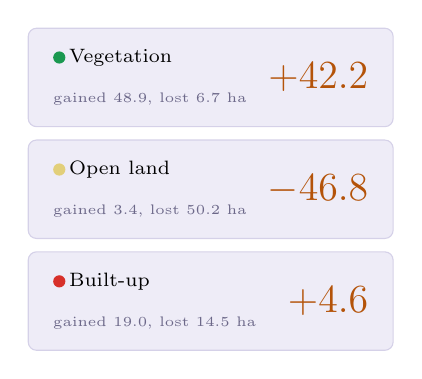
\begin{tikzpicture}
  \foreach \n/\c/\a/\b/\d [count=\i] in {Vegetation/cveg/48.9/6.7/+42.2,Open land/copen/3.4/50.2/$-$46.8,Built-up/cbuilt/19.0/14.5/+4.6}{
    \node[card,text width=4.4cm,minimum height=1.25cm,anchor=north west] (k\i) at (0,-1.42*\i) {};
    \node[anchor=north west,font=\scriptsize] at ([xshift=2mm,yshift=-1.5mm]k\i.north west) {\sw{\c}\,\n};
    \node[anchor=south west,font=\tiny,text=muted] at ([xshift=2mm,yshift=1.5mm]k\i.south west) {gained \a, lost \b\ ha};
    \node[anchor=east] at ([xshift=-2mm]k\i.east) {{\color{saffron}\fontsize{15}{17}\selectfont\d}};
  }
\end{tikzpicture}\\[2mm]
{\scriptsize\textbf{Map vs points.} The point estimate (Olofsson et al. 2014) corrects for known map errors. Mapped open land sits 43 ha (2020) and 39 ha (2025) below it. Built-up: map +4.6, points $-$41 $\pm$ 45 ha; neither is distinguishable from zero. Only vegetation's intervals do not overlap (169-272 vs 273-356 ha).}
\end{column}
\end{columns}
\end{frame}

% ---------------------------------------------------------------- flows, gain, loss, swap
\begin{frame}{Open land feeds both vegetation and building; built-up mostly swaps place}{CHANGE FLOW \textperiodcentered\ GROSS GAIN, LOSS AND SWAP}
\begin{columns}[T]
\begin{column}{.54\textwidth}\centering
\resizebox{\linewidth}{!}{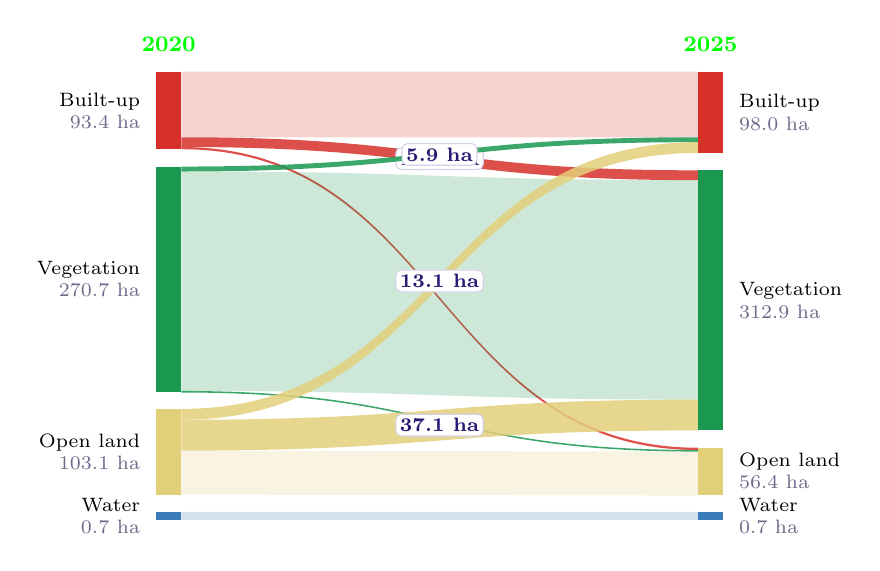
\begin{tikzpicture}\fill[cbuilt,opacity=0.22] (0.32,5.600) .. controls (3.6,5.600) and (3.6,5.600) .. (6.88,5.600) -- (6.88,4.766) .. controls (3.6,4.766) and (3.6,4.766) .. (0.32,4.766) -- cycle;
\fill[cbuilt,opacity=0.85] (0.32,4.766) .. controls (3.6,4.766) and (3.6,4.346) .. (6.88,4.346) -- (6.88,4.221) .. controls (3.6,4.221) and (3.6,4.642) .. (0.32,4.642) -- cycle;
\node[font=\scriptsize\bfseries,text=ink,fill=white,draw=rule,inner sep=1.5pt,rounded corners=2pt] at (3.6,4.494) {11.8 ha};
\fill[cbuilt,opacity=0.85] (0.32,4.642) .. controls (3.6,4.642) and (3.6,0.823) .. (6.88,0.823) -- (6.88,0.794) .. controls (3.6,0.794) and (3.6,4.614) .. (0.32,4.614) -- cycle;
\fill[cveg,opacity=0.85] (0.32,4.394) .. controls (3.6,4.394) and (3.6,4.766) .. (6.88,4.766) -- (6.88,4.704) .. controls (3.6,4.704) and (3.6,4.331) .. (0.32,4.331) -- cycle;
\node[font=\scriptsize\bfseries,text=ink,fill=white,draw=rule,inner sep=1.5pt,rounded corners=2pt] at (3.6,4.549) {5.9 ha};
\fill[cveg,opacity=0.22] (0.32,4.331) .. controls (3.6,4.331) and (3.6,4.221) .. (6.88,4.221) -- (6.88,1.434) .. controls (3.6,1.434) and (3.6,1.544) .. (0.32,1.544) -- cycle;
\fill[cveg,opacity=0.85] (0.32,1.544) .. controls (3.6,1.544) and (3.6,0.794) .. (6.88,0.794) -- (6.88,0.774) .. controls (3.6,0.774) and (3.6,1.524) .. (0.32,1.524) -- cycle;
\fill[copen,opacity=0.85] (0.32,1.316) .. controls (3.6,1.316) and (3.6,4.704) .. (6.88,4.704) -- (6.88,4.566) .. controls (3.6,4.566) and (3.6,1.178) .. (0.32,1.178) -- cycle;
\node[font=\scriptsize\bfseries,text=ink,fill=white,draw=rule,inner sep=1.5pt,rounded corners=2pt] at (3.6,2.941) {13.1 ha};
\fill[copen,opacity=0.85] (0.32,1.178) .. controls (3.6,1.178) and (3.6,1.434) .. (6.88,1.434) -- (6.88,1.043) .. controls (3.6,1.043) and (3.6,0.786) .. (0.32,0.786) -- cycle;
\node[font=\scriptsize\bfseries,text=ink,fill=white,draw=rule,inner sep=1.5pt,rounded corners=2pt] at (3.6,1.110) {37.1 ha};
\fill[copen,opacity=0.22] (0.32,0.786) .. controls (3.6,0.786) and (3.6,0.774) .. (6.88,0.774) -- (6.88,0.215) .. controls (3.6,0.215) and (3.6,0.228) .. (0.32,0.228) -- cycle;
\fill[cwater,opacity=0.22] (0.32,0.008) .. controls (3.6,0.008) and (3.6,0.008) .. (6.88,0.008) -- (6.88,-0.092) .. controls (3.6,-0.092) and (3.6,-0.092) .. (0.32,-0.092) -- cycle;
\fill[cbuilt] (0,5.600) rectangle (0.32,4.614);
\fill[cbuilt] (6.88,5.600) rectangle (7.2,4.566);
\node[anchor=east,font=\scriptsize,align=right] at (-0.08,5.107) {Built-up\\\textcolor{muted}{93.4 ha}};
\node[anchor=west,font=\scriptsize,align=left] at (7.28,5.083) {Built-up\\\textcolor{muted}{98.0 ha}};
\fill[cveg] (0,4.394) rectangle (0.32,1.536);
\fill[cveg] (6.88,4.346) rectangle (7.2,1.043);
\node[anchor=east,font=\scriptsize,align=right] at (-0.08,2.965) {Vegetation\\\textcolor{muted}{270.7 ha}};
\node[anchor=west,font=\scriptsize,align=left] at (7.28,2.694) {Vegetation\\\textcolor{muted}{312.9 ha}};
\fill[copen] (0,1.316) rectangle (0.32,0.228);
\fill[copen] (6.88,0.823) rectangle (7.2,0.228);
\node[anchor=east,font=\scriptsize,align=right] at (-0.08,0.772) {Open land\\\textcolor{muted}{103.1 ha}};
\node[anchor=west,font=\scriptsize,align=left] at (7.28,0.525) {Open land\\\textcolor{muted}{56.4 ha}};
\fill[cwater] (0,0.008) rectangle (0.32,-0.092);
\fill[cwater] (6.88,0.008) rectangle (7.2,-0.092);
\node[anchor=east,font=\scriptsize,align=right] at (-0.08,-0.042) {Water\\\textcolor{muted}{0.7 ha}};
\node[anchor=west,font=\scriptsize,align=left] at (7.28,-0.042) {Water\\\textcolor{muted}{0.7 ha}};
\node[font=\footnotesize\bfseries,text=green] at (0.16,5.949999999999999) {2020};
\node[font=\footnotesize\bfseries,text=green] at (7.04,5.949999999999999) {2025};
\end{tikzpicture}}\\[1mm]
\capt{Band width = hectares; faint bands stayed the same class. From-to table after the 30 m filter.}
\end{column}
\begin{column}{.43\textwidth}
{\footnotesize\begin{tabular}{@{}lrrrr@{}}
\toprule
ha & gained & lost & net & swap \\
\midrule
\sw{cbuilt}\,Built-up & 19.0 & 14.5 & \textbf{+4.6} & 29.0 \\
\sw{cveg}\,Vegetation & 48.9 & 6.7 & \textbf{+42.2} & 13.3 \\
\sw{copen}\,Open land & 3.4 & 50.2 & \textbf{$-$46.8} & 6.9 \\
\bottomrule
\end{tabular}
}\\[1mm]
{\tiny\color{muted}Swap = 2 $\times$ min(gain, loss): area that changed place without changing the class total (Pontius et al. 2004).}\\[2mm]
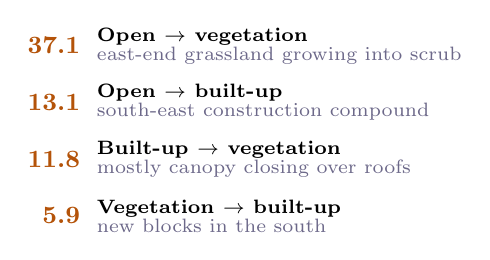
\begin{tikzpicture}
  \foreach \v/\t/\d [count=\i] in {37.1/Open \ra{} vegetation/east-end grassland growing into scrub,13.1/Open \ra{} built-up/south-east construction compound,11.8/Built-up \ra{} vegetation/mostly canopy closing over roofs,5.9/Vegetation \ra{} built-up/new blocks in the south}{
    \node[anchor=east,inner sep=0] at (1.0,-.72*\i) {{\color{saffron}\small\bfseries\v}};
    \node[anchor=west,font=\scriptsize,inner sep=0,align=left] at (1.2,-.72*\i) {\textbf{\t}\\[-.4mm]{\color{muted}\d}};
  }
\end{tikzpicture}\\[2mm]
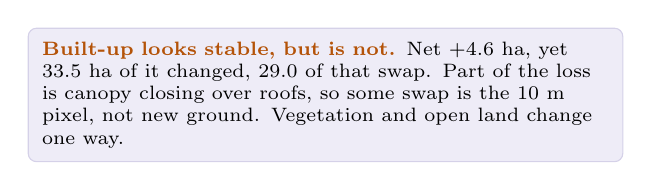
\begin{tikzpicture}
  \node[card,text width=7.2cm,inner sep=5pt,font=\scriptsize] {{\color{saffron}\bfseries Built-up looks stable, but is not.} Net +4.6 ha, yet 33.5 ha of it changed, 29.0 of that swap. Part of the loss is canopy closing over roofs, so some swap is the 10 m pixel, not new ground. Vegetation and open land change one way.};
\end{tikzpicture}
\end{column}
\end{columns}
\end{frame}

% ---------------------------------------------------------------- dating the compound (new)
\begin{frame}{The south-east compound was cleared in 2020 and had roofs by early 2023}{NEW ANALYSIS: ONE COMPOSITE PER WINTER, SAME FOREST}
\centering
\begin{tikzpicture}\node[anchor=north west,inner sep=0] (c0) at (0.00,0) {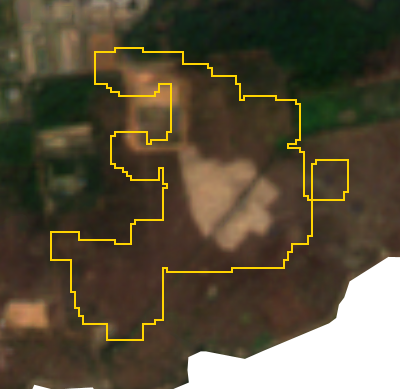
\includegraphics[width=2.7cm]{img/compound_2020.png}};
\node[anchor=north west,font=\scriptsize\bfseries,inner sep=0] at ([yshift=-1.5mm]c0.south west) {2019-20};
\fill[copen] (0.000,-3.23) rectangle (2.700,-3.45);
\node[anchor=north east,font=\scriptsize\bfseries,text=saffron,inner sep=0] at ([yshift=-1.5mm]c0.south east) {0\% built};
\node[anchor=north west,inner sep=0] (c1) at (2.95,0) {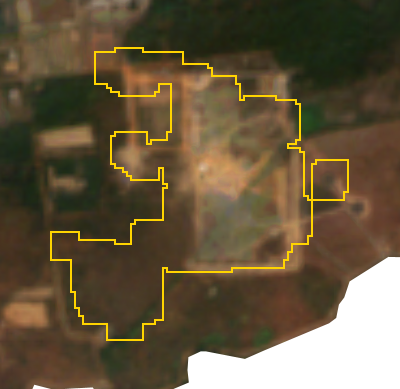
\includegraphics[width=2.7cm]{img/compound_2021.png}};
\node[anchor=north west,font=\scriptsize\bfseries,inner sep=0] at ([yshift=-1.5mm]c1.south west) {2020-21};
\fill[cbuilt] (2.950,-3.23) rectangle (3.283,-3.45);
\fill[cveg] (3.283,-3.23) rectangle (3.298,-3.45);
\fill[copen] (3.298,-3.23) rectangle (5.652,-3.45);
\node[anchor=north east,font=\scriptsize\bfseries,text=saffron,inner sep=0] at ([yshift=-1.5mm]c1.south east) {12\% built};
\node[anchor=north west,inner sep=0] (c2) at (5.90,0) {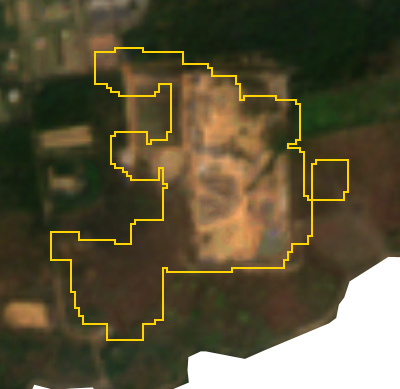
\includegraphics[width=2.7cm]{img/compound_2022.png}};
\node[anchor=north west,font=\scriptsize\bfseries,inner sep=0] at ([yshift=-1.5mm]c2.south west) {2021-22};
\fill[cbuilt] (5.900,-3.23) rectangle (6.928,-3.45);
\fill[cveg] (6.928,-3.23) rectangle (7.455,-3.45);
\fill[copen] (7.455,-3.23) rectangle (8.602,-3.45);
\node[anchor=north east,font=\scriptsize\bfseries,text=saffron,inner sep=0] at ([yshift=-1.5mm]c2.south east) {38\% built};
\node[anchor=north west,inner sep=0] (c3) at (8.85,0) {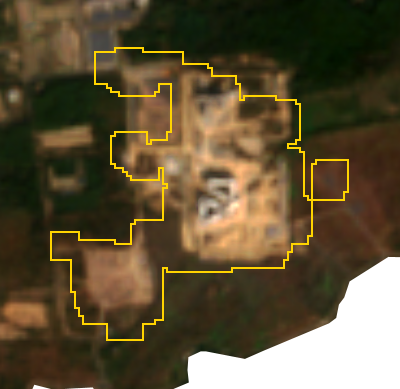
\includegraphics[width=2.7cm]{img/compound_2023.png}};
\node[anchor=north west,font=\scriptsize\bfseries,inner sep=0] at ([yshift=-1.5mm]c3.south west) {2022-23};
\fill[cbuilt] (8.850,-3.23) rectangle (10.908,-3.45);
\fill[cveg] (10.908,-3.23) rectangle (10.923,-3.45);
\fill[copen] (10.923,-3.23) rectangle (11.548,-3.45);
\node[anchor=north east,font=\scriptsize\bfseries,text=saffron,inner sep=0] at ([yshift=-1.5mm]c3.south east) {76\% built};
\node[anchor=north west,inner sep=0] (c4) at (11.80,0) {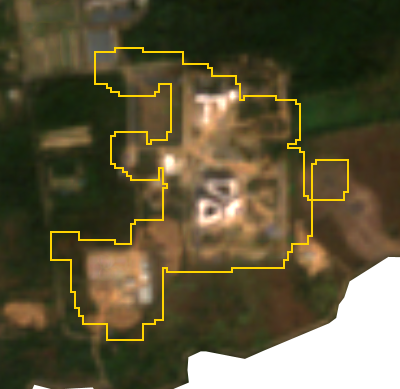
\includegraphics[width=2.7cm]{img/compound_2024.png}};
\node[anchor=north west,font=\scriptsize\bfseries,inner sep=0] at ([yshift=-1.5mm]c4.south west) {2023-24};
\fill[cbuilt] (11.800,-3.23) rectangle (13.530,-3.45);
\fill[cveg] (13.530,-3.23) rectangle (13.633,-3.45);
\fill[copen] (13.633,-3.23) rectangle (14.500,-3.45);
\node[anchor=north east,font=\scriptsize\bfseries,text=saffron,inner sep=0] at ([yshift=-1.5mm]c4.south east) {64\% built};
\node[anchor=north west,inner sep=0] (c5) at (14.75,0) {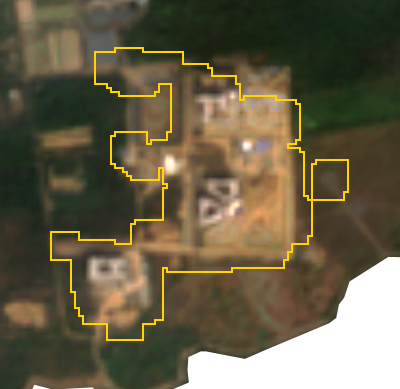
\includegraphics[width=2.7cm]{img/compound_2025.png}};
\node[anchor=north west,font=\scriptsize\bfseries,inner sep=0] at ([yshift=-1.5mm]c5.south west) {2024-25};
\fill[cbuilt] (14.750,-3.23) rectangle (17.450,-3.45);
\node[anchor=north east,font=\scriptsize\bfseries,text=saffron,inner sep=0] at ([yshift=-1.5mm]c5.south east) {100\% built};
\end{tikzpicture}\\[1.5mm]
{\scriptsize\color{muted}Winter true colour, site in yellow. Bar: the forest's class for the site's open \ra{} built-up pixels \quad \sw{cbuilt}\,built-up \quad \sw{cveg}\,vegetation \quad \sw{copen}\,open land}\\[3mm]
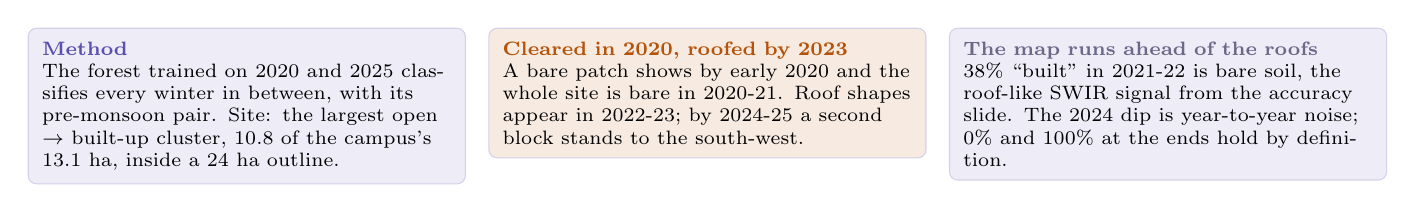
\begin{tikzpicture}
  \node[card,text width=5.2cm,inner sep=5pt,font=\scriptsize,anchor=north west] at (0,0) {{\color{iris}\bfseries Method}\\The forest trained on 2020 and 2025 classifies every winter in between, with its pre-monsoon pair. Site: the largest open \ra{} built-up cluster, 10.8 of the campus's 13.1 ha, inside a 24 ha outline.};
  \node[card,text width=5.2cm,inner sep=5pt,font=\scriptsize,anchor=north west,fill=saffron!12] at (5.85,0) {{\color{saffron}\bfseries Cleared in 2020, roofed by 2023}\\A bare patch shows by early 2020 and the whole site is bare in 2020-21. Roof shapes appear in 2022-23; by 2024-25 a second block stands to the south-west.};
  \node[card,text width=5.2cm,inner sep=5pt,font=\scriptsize,anchor=north west] at (11.7,0) {{\color{muted}\bfseries The map runs ahead of the roofs}\\38\% ``built'' in 2021-22 is bare soil, the roof-like SWIR signal from the accuracy slide. The 2024 dip is year-to-year noise; 0\% and 100\% at the ends hold by definition.};
\end{tikzpicture}
\end{frame}

% ---------------------------------------------------------------- worldview validation
\begin{frame}{Validation labels come from WorldView, 20 times sharper than Sentinel-2}{ACCURACY ASSESSMENT DESIGN}
\begin{columns}[T]
\begin{column}{.3\textwidth}
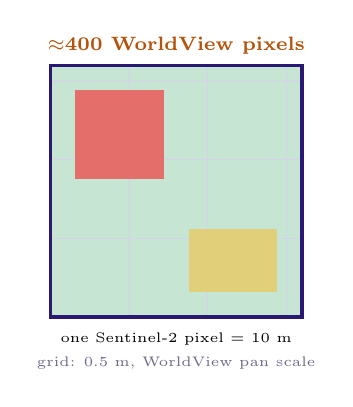
\begin{tikzpicture}
  \fill[cveg!25] (0,0) rectangle (3.2,3.2);
  \draw[step=.16,rule,line width=.15pt] (0,0) grid (3.2,3.2);
  \draw[ink,line width=1.2pt] (0,0) rectangle (3.2,3.2);
  \fill[cbuilt!70] (.32,1.76) rectangle (1.44,2.88);
  \fill[copen] (1.76,.32) rectangle (2.88,1.12);
  \node[font=\tiny,anchor=north] at (1.6,-.08) {one Sentinel-2 pixel = 10 m};
  \node[font=\tiny,anchor=north,text=muted] at (1.6,-.38) {grid: 0.5 m, WorldView pan scale};
  \node[font=\scriptsize\bfseries,text=saffron] at (1.6,3.45) {$\approx$400 WorldView pixels};
\end{tikzpicture}\\[3mm]
{\scriptsize A 10 m pixel that mixes a roof and a lawn is one label to the classifier but readable by eye on WorldView.}
\end{column}
\begin{column}{.67\textwidth}
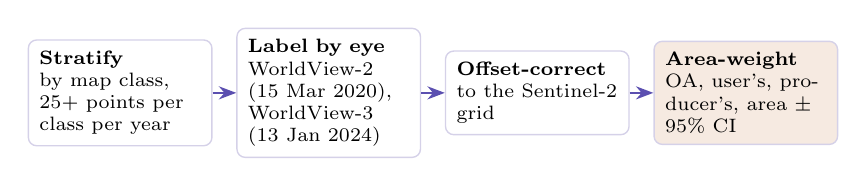
\begin{tikzpicture}[node distance=3mm]
  \node[step=2.05cm] (v1) {\textbf{Stratify}\\by map class, 25+ points per class per year};
  \node[step=2.05cm,right=of v1] (v2) {\textbf{Label by eye}\\WorldView-2 (15 Mar 2020), WorldView-3 (13 Jan 2024)};
  \node[step=2.05cm,right=of v2] (v3) {\textbf{Offset-correct}\\to the Sentinel-2 grid};
  \node[step=2.05cm,right=of v3,fill=saffron!12] (v4) {\textbf{Area-weight}\\OA, user's, producer's, area $\pm$ 95\% CI};
  \foreach \a/\b in {v1/v2,v2/v3,v3/v4}{\draw[flowarrow] (\a) -- (\b);}
\end{tikzpicture}\\[3mm]
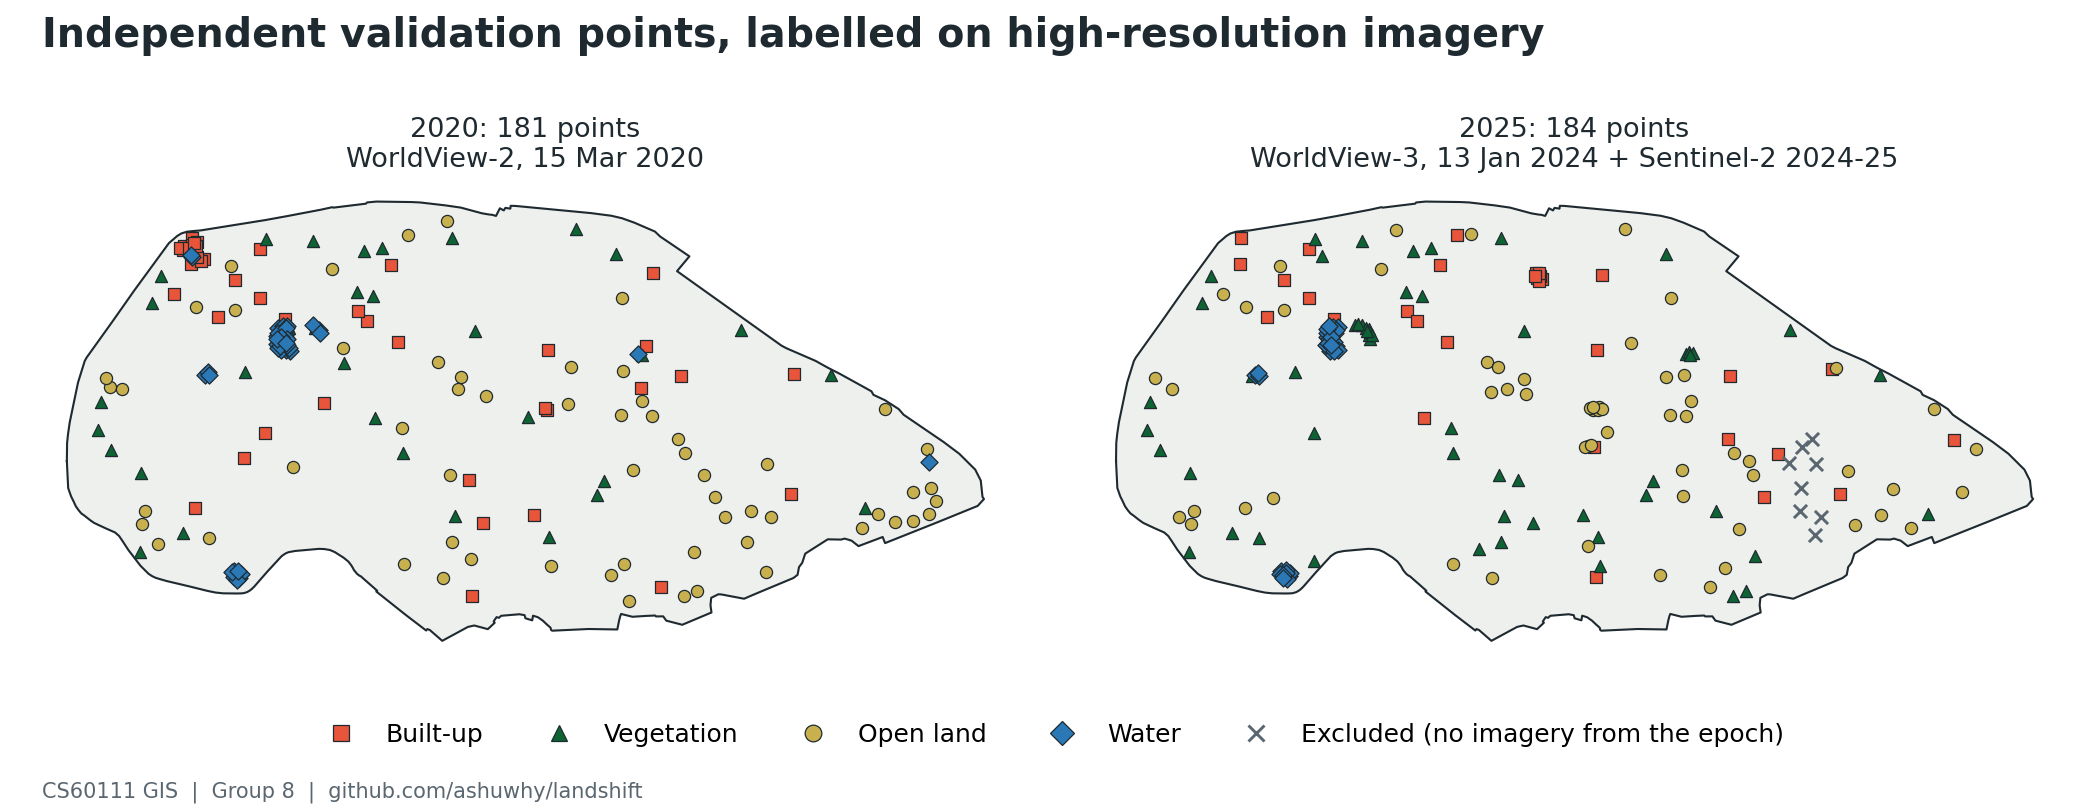
\includegraphics[width=\linewidth]{img/08_validation_points.png}\\
\capt{365 points: 181 for 2020, 184 for 2025, labelled by Krishnkant Sahu. Independent of Dynamic World, unlike the 883 held-out training pixels.}
\end{column}
\end{columns}
\end{frame}

% ---------------------------------------------------------------- accuracy and confusion
\begin{frame}{Accuracy 0.67 (2020) and 0.77 (2025); open land is the weak class}{ACCURACY, INDEPENDENT WORLDVIEW POINTS}
\begin{columns}[T]
\begin{column}{.33\textwidth}
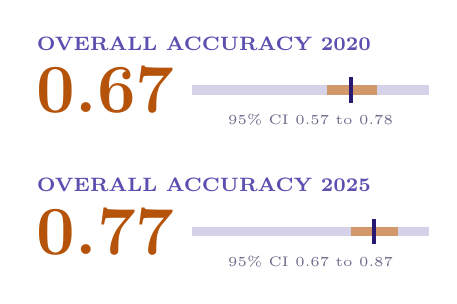
\begin{tikzpicture}
  \foreach \y/\oa/\lo/\hi/\yr in {0/0.67/0.57/0.78/2020,-1.8/0.77/0.67/0.87/2025}{
    \node[anchor=west] at (0,\y+.35) {\capt{OVERALL ACCURACY \yr}};
    \node[anchor=west] at (0,\y-.25) {{\color{saffron}\fontsize{24}{26}\selectfont\bfseries\oa}};
    \fill[rule] (2.1,\y-.3) rectangle (5.1,\y-.18);
    \fill[saffron!60] (2.1+3*\lo,\y-.3) rectangle (2.1+3*\hi,\y-.18);
    \draw[ink,line width=1.4pt] (2.1+3*\oa,\y-.4) -- (2.1+3*\oa,\y-.08);
    \node[font=\tiny,text=muted,anchor=north] at (3.6,\y-.42) {95\% CI \lo\ to \hi};
  }
\end{tikzpicture}\\[2mm]
{\scriptsize Area-weighted (Olofsson et al. 2014). Against Dynamic World's own held-out pixels the map scores 0.82 / 0.88 (kappa 0.73 / 0.81), but that only measures agreement with the training source.}\\[2mm]
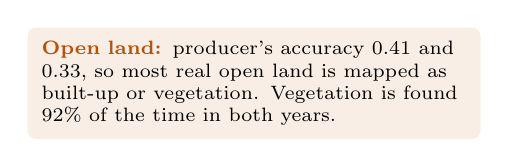
\begin{tikzpicture}
  \node[fill=saffron!10,rounded corners=3pt,text width=5.4cm,inner sep=5pt,font=\scriptsize] {\textbf{\color{saffron}Open land:} producer's accuracy 0.41 and 0.33, so most real open land is mapped as built-up or vegetation. Vegetation is found 92\% of the time in both years.};
\end{tikzpicture}
\end{column}
\begin{column}{.64\textwidth}\centering
\resizebox{.94\linewidth}{!}{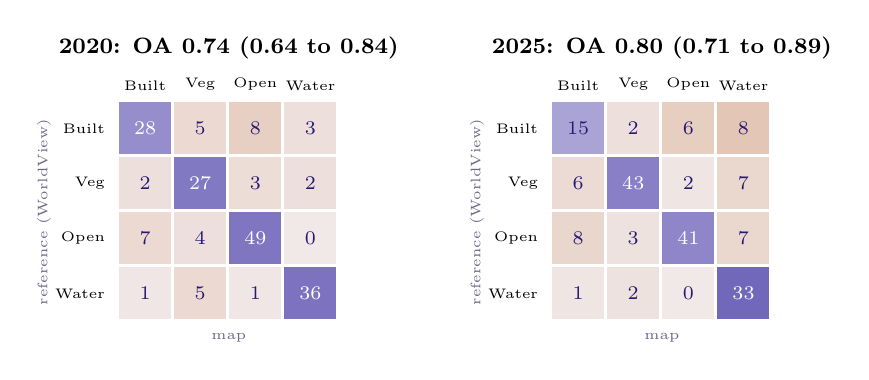
\begin{tikzpicture}
  \begin{scope}[xshift=.9cm]\fill[iris!62!bg] (0.000,0.000) rectangle (0.660,-0.660);
\node[font=\scriptsize,text=white] at (0.336,-0.336) {28};
\fill[saffron!17!bg] (0.700,0.000) rectangle (1.360,-0.660);
\node[font=\scriptsize,text=ink] at (1.036,-0.336) {5};
\fill[saffron!23!bg] (1.400,0.000) rectangle (2.060,-0.660);
\node[font=\scriptsize,text=ink] at (1.736,-0.336) {8};
\fill[saffron!13!bg] (2.100,0.000) rectangle (2.760,-0.660);
\node[font=\scriptsize,text=ink] at (2.436,-0.336) {3};
\node[anchor=east,font=\tiny] at (-0.05,-0.336) {Built};
\node[anchor=south,font=\tiny] at (0.336,0.02) {Built};
\fill[saffron!13!bg] (0.000,-0.700) rectangle (0.660,-1.360);
\node[font=\scriptsize,text=ink] at (0.336,-1.036) {2};
\fill[iris!75!bg] (0.700,-0.700) rectangle (1.360,-1.360);
\node[font=\scriptsize,text=white] at (1.036,-1.036) {27};
\fill[saffron!15!bg] (1.400,-0.700) rectangle (2.060,-1.360);
\node[font=\scriptsize,text=ink] at (1.736,-1.036) {3};
\fill[saffron!13!bg] (2.100,-0.700) rectangle (2.760,-1.360);
\node[font=\scriptsize,text=ink] at (2.436,-1.036) {2};
\node[anchor=east,font=\tiny] at (-0.05,-1.036) {Veg};
\node[anchor=south,font=\tiny] at (1.036,0.02) {Veg};
\fill[saffron!17!bg] (0.000,-1.400) rectangle (0.660,-2.060);
\node[font=\scriptsize,text=ink] at (0.336,-1.736) {7};
\fill[saffron!13!bg] (0.700,-1.400) rectangle (1.360,-2.060);
\node[font=\scriptsize,text=ink] at (1.036,-1.736) {4};
\fill[iris!77!bg] (1.400,-1.400) rectangle (2.060,-2.060);
\node[font=\scriptsize,text=white] at (1.736,-1.736) {49};
\fill[saffron!8!bg] (2.100,-1.400) rectangle (2.760,-2.060);
\node[font=\scriptsize,text=ink] at (2.436,-1.736) {0};
\node[anchor=east,font=\tiny] at (-0.05,-1.736) {Open};
\node[anchor=south,font=\tiny] at (1.736,0.02) {Open};
\fill[saffron!9!bg] (0.000,-2.100) rectangle (0.660,-2.760);
\node[font=\scriptsize,text=ink] at (0.336,-2.436) {1};
\fill[saffron!17!bg] (0.700,-2.100) rectangle (1.360,-2.760);
\node[font=\scriptsize,text=ink] at (1.036,-2.436) {5};
\fill[saffron!9!bg] (1.400,-2.100) rectangle (2.060,-2.760);
\node[font=\scriptsize,text=ink] at (1.736,-2.436) {1};
\fill[iris!79!bg] (2.100,-2.100) rectangle (2.760,-2.760);
\node[font=\scriptsize,text=white] at (2.436,-2.436) {36};
\node[anchor=east,font=\tiny] at (-0.05,-2.436) {Water};
\node[anchor=south,font=\tiny] at (2.436,0.02) {Water};
\node[font=\footnotesize\bfseries,anchor=south] at (1.400,0.42) {2020: OA 0.74 (0.64 to 0.84)};
\node[font=\tiny,text=muted,rotate=90] at (-0.95,-1.400) {reference (WorldView)};
\node[font=\tiny,text=muted] at (1.400,-3.000) {map};
\end{scope}
  \begin{scope}[xshift=6.4cm]\fill[iris!49!bg] (0.000,0.000) rectangle (0.660,-0.660);
\node[font=\scriptsize,text=ink] at (0.336,-0.336) {15};
\fill[saffron!13!bg] (0.700,0.000) rectangle (1.360,-0.660);
\node[font=\scriptsize,text=ink] at (1.036,-0.336) {2};
\fill[saffron!24!bg] (1.400,0.000) rectangle (2.060,-0.660);
\node[font=\scriptsize,text=ink] at (1.736,-0.336) {6};
\fill[saffron!29!bg] (2.100,0.000) rectangle (2.760,-0.660);
\node[font=\scriptsize,text=ink] at (2.436,-0.336) {8};
\node[anchor=east,font=\tiny] at (-0.05,-0.336) {Built};
\node[anchor=south,font=\tiny] at (0.336,0.02) {Built};
\fill[saffron!16!bg] (0.000,-0.700) rectangle (0.660,-1.360);
\node[font=\scriptsize,text=ink] at (0.336,-1.036) {6};
\fill[iris!71!bg] (0.700,-0.700) rectangle (1.360,-1.360);
\node[font=\scriptsize,text=white] at (1.036,-1.036) {43};
\fill[saffron!10!bg] (1.400,-0.700) rectangle (2.060,-1.360);
\node[font=\scriptsize,text=ink] at (1.736,-1.036) {2};
\fill[saffron!18!bg] (2.100,-0.700) rectangle (2.760,-1.360);
\node[font=\scriptsize,text=ink] at (2.436,-1.036) {7};
\node[anchor=east,font=\tiny] at (-0.05,-1.036) {Veg};
\node[anchor=south,font=\tiny] at (1.036,0.02) {Veg};
\fill[saffron!19!bg] (0.000,-1.400) rectangle (0.660,-2.060);
\node[font=\scriptsize,text=ink] at (0.336,-1.736) {8};
\fill[saffron!12!bg] (0.700,-1.400) rectangle (1.360,-2.060);
\node[font=\scriptsize,text=ink] at (1.036,-1.736) {3};
\fill[iris!67!bg] (1.400,-1.400) rectangle (2.060,-2.060);
\node[font=\scriptsize,text=white] at (1.736,-1.736) {41};
\fill[saffron!18!bg] (2.100,-1.400) rectangle (2.760,-2.060);
\node[font=\scriptsize,text=ink] at (2.436,-1.736) {7};
\node[anchor=east,font=\tiny] at (-0.05,-1.736) {Open};
\node[anchor=south,font=\tiny] at (1.736,0.02) {Open};
\fill[saffron!10!bg] (0.000,-2.100) rectangle (0.660,-2.760);
\node[font=\scriptsize,text=ink] at (0.336,-2.436) {1};
\fill[saffron!12!bg] (0.700,-2.100) rectangle (1.360,-2.760);
\node[font=\scriptsize,text=ink] at (1.036,-2.436) {2};
\fill[saffron!8!bg] (1.400,-2.100) rectangle (2.060,-2.760);
\node[font=\scriptsize,text=ink] at (1.736,-2.436) {0};
\fill[iris!85!bg] (2.100,-2.100) rectangle (2.760,-2.760);
\node[font=\scriptsize,text=white] at (2.436,-2.436) {33};
\node[anchor=east,font=\tiny] at (-0.05,-2.436) {Water};
\node[anchor=south,font=\tiny] at (2.436,0.02) {Water};
\node[font=\footnotesize\bfseries,anchor=south] at (1.400,0.42) {2025: OA 0.80 (0.71 to 0.89)};
\node[font=\tiny,text=muted,rotate=90] at (-0.95,-1.400) {reference (WorldView)};
\node[font=\tiny,text=muted] at (1.400,-3.000) {map};
\end{scope}
\end{tikzpicture}}\\[1mm]
\capt{Point counts. Rows: WorldView reference; columns: map. Shade: share of the row; indigo diagonal is correct, saffron is error.}\\[2mm]
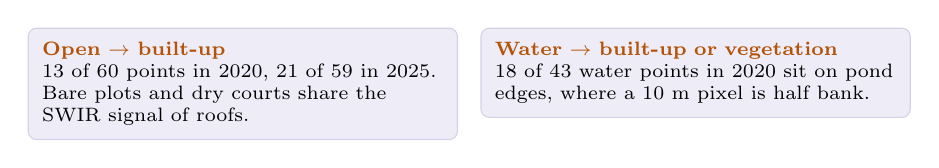
\begin{tikzpicture}
  \node[card,text width=5.1cm,inner sep=5pt,font=\scriptsize,anchor=north west] at (0,0) {{\color{saffron}\bfseries Open \ra{} built-up}\\13 of 60 points in 2020, 21 of 59 in 2025. Bare plots and dry courts share the SWIR signal of roofs.};
  \node[card,text width=5.1cm,inner sep=5pt,font=\scriptsize,anchor=north west] at (5.75,0) {{\color{saffron}\bfseries Water \ra{} built-up or vegetation}\\18 of 43 water points in 2020 sit on pond edges, where a 10 m pixel is half bank.};
\end{tikzpicture}
\end{column}
\end{columns}
\end{frame}

% ---------------------------------------------------------------- significance (new)
\begin{frame}{Only the vegetation gain is bigger than our map error}{NEW ANALYSIS: IS THE CHANGE STATISTICALLY REAL?}
\centering
\capt{ERROR-ADJUSTED NET CHANGE 2020 \ra{} 2025 WITH 95\% CI \qquad $\bullet$ point-based estimate \qquad $\diamond$ map, from-to net}\\[2mm]
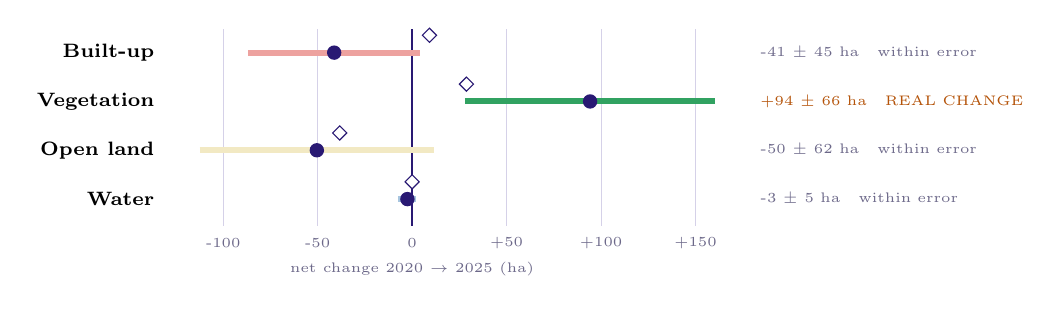
\begin{tikzpicture}\draw[rule] (-2.40,.3) -- (-2.40,-2.2);
\node[font=\tiny,text=muted] at (-2.40,-2.42) {-100};
\draw[rule] (-1.20,.3) -- (-1.20,-2.2);
\node[font=\tiny,text=muted] at (-1.20,-2.42) {-50};
\draw[ink,thick] (0.00,.3) -- (0.00,-2.2);
\node[font=\tiny,text=muted] at (0.00,-2.42) {0};
\draw[rule] (1.20,.3) -- (1.20,-2.2);
\node[font=\tiny,text=muted] at (1.20,-2.42) {+50};
\draw[rule] (2.40,.3) -- (2.40,-2.2);
\node[font=\tiny,text=muted] at (2.40,-2.42) {+100};
\draw[rule] (3.60,.3) -- (3.60,-2.2);
\node[font=\tiny,text=muted] at (3.60,-2.42) {+150};
\node[anchor=east,font=\scriptsize\bfseries] at (-3.15,-0.0) {Built-up};
\draw[line width=2.2pt,cbuilt!45] (-2.08,-0.0) -- (0.10,-0.0);
\fill[ink] (-0.99,-0.0) circle (2.6pt);
\draw[ink,fill=white] (0.22,0.22) +(0,.09) -- +(.09,0) -- +(0,-.09) -- +(-.09,0) -- cycle;
\node[anchor=west,font=\tiny,text=muted] at (4.3,-0.0) {-41 $\pm$ 45 ha \; within error};
\node[anchor=east,font=\scriptsize\bfseries] at (-3.15,-0.62) {Vegetation};
\draw[line width=2.2pt,cveg!90] (0.67,-0.62) -- (3.85,-0.62);
\fill[ink] (2.26,-0.62) circle (2.6pt);
\draw[ink,fill=white] (0.69,-0.4) +(0,.09) -- +(.09,0) -- +(0,-.09) -- +(-.09,0) -- cycle;
\node[anchor=west,font=\tiny,text=saffron] at (4.3,-0.62) {+94 $\pm$ 66 ha \; REAL CHANGE};
\node[anchor=east,font=\scriptsize\bfseries] at (-3.15,-1.24) {Open land};
\draw[line width=2.2pt,copen!45] (-2.70,-1.24) -- (0.28,-1.24);
\fill[ink] (-1.21,-1.24) circle (2.6pt);
\draw[ink,fill=white] (-0.92,-1.02) +(0,.09) -- +(.09,0) -- +(0,-.09) -- +(-.09,0) -- cycle;
\node[anchor=west,font=\tiny,text=muted] at (4.3,-1.24) {-50 $\pm$ 62 ha \; within error};
\node[anchor=east,font=\scriptsize\bfseries] at (-3.15,-1.8599999999999999) {Water};
\draw[line width=2.2pt,cwater!45] (-0.18,-1.8599999999999999) -- (0.05,-1.8599999999999999);
\fill[ink] (-0.06,-1.8599999999999999) circle (2.6pt);
\draw[ink,fill=white] (0.00,-1.64) +(0,.09) -- +(.09,0) -- +(0,-.09) -- +(-.09,0) -- cycle;
\node[anchor=west,font=\tiny,text=muted] at (4.3,-1.8599999999999999) {-3 $\pm$ 5 ha \; within error};
\node[font=\tiny,text=muted] at (0,-2.75) {net change 2020 $\rightarrow$ 2025 (ha)};
\end{tikzpicture}\\[2mm]
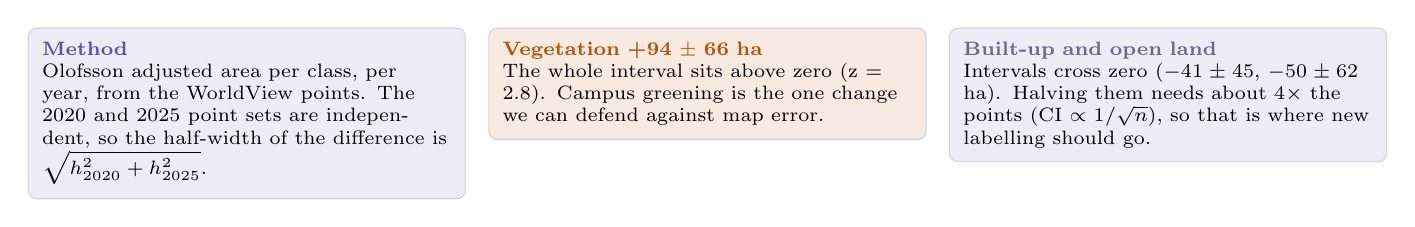
\begin{tikzpicture}
  \node[card,text width=5.2cm,inner sep=5pt,font=\scriptsize,anchor=north west] (m) at (0,0) {{\color{iris}\bfseries Method}\\Olofsson adjusted area per class, per year, from the WorldView points. The 2020 and 2025 point sets are independent, so the half-width of the difference is $\sqrt{h_{2020}^2+h_{2025}^2}$.};
  \node[card,text width=5.2cm,inner sep=5pt,font=\scriptsize,anchor=north west,fill=saffron!12] (v) at (5.85,0) {{\color{saffron}\bfseries Vegetation +94 $\pm$ 66 ha}\\The whole interval sits above zero (z = 2.8). Campus greening is the one change we can defend against map error.};
  \node[card,text width=5.2cm,inner sep=5pt,font=\scriptsize,anchor=north west] (b) at (11.7,0) {{\color{muted}\bfseries Built-up and open land}\\Intervals cross zero ($-41 \pm 45$, $-50 \pm 62$ ha). Halving them needs about 4$\times$ the points (CI $\propto 1/\sqrt{n}$), so that is where new labelling should go.};
\end{tikzpicture}
\end{frame}

% ---------------------------------------------------------------- conclusions and limits
\begin{frame}{15.2\% of the campus changed, mostly open land turning green}{CONCLUSIONS, LIMITS AND NEXT STEPS}
\begin{columns}[T]
\begin{column}{.38\textwidth}
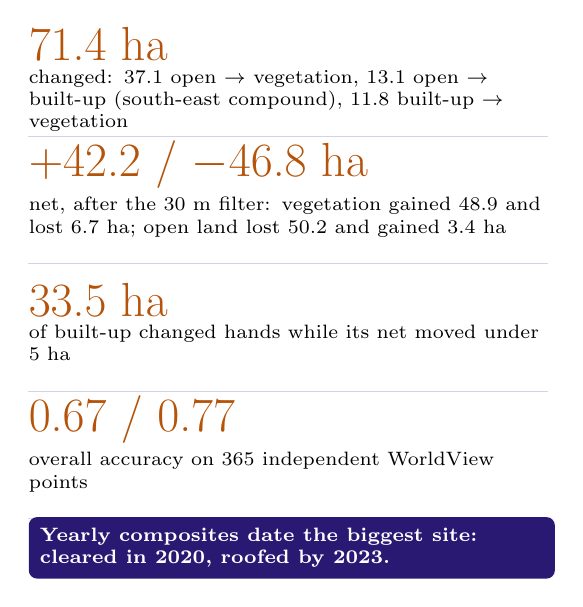
\begin{tikzpicture}
  \foreach \v/\t [count=\i] in {71.4 ha/changed: 37.1 open \ra{} vegetation{,} 13.1 open \ra{} built-up (south-east compound){,} 11.8 built-up \ra{} vegetation,{+42.2 / $-$46.8 ha}/net{,} after the 30 m filter: vegetation gained 48.9 and lost 6.7 ha; open land lost 50.2 and gained 3.4 ha,33.5 ha/of built-up changed hands while its net moved under 5 ha,{0.67 / 0.77}/overall accuracy on 365 independent WorldView points}{
    \node[anchor=south west,inner sep=0] at (0,-1.62*\i) {{\color{saffron}\fontsize{16}{18}\selectfont\v}};
    \node[anchor=north west,inner sep=0,text width=6.6cm,font=\scriptsize] at (0,-1.62*\i-.1) {\t};
    \draw[rule] (0,-1.62*\i-.95) -- (6.6,-1.62*\i-.95);
  }
  \node[fill=ink,text=white,rounded corners=3pt,text width=6.4cm,inner sep=4pt,font=\scriptsize\bfseries,anchor=north west] at (0,-7.4) {Yearly composites date the biggest site: cleared in 2020, roofed by 2023.};
\end{tikzpicture}
\end{column}
\begin{column}{.59\textwidth}
\capt{WHAT THE MAP CANNOT SUPPORT}\\[1.5mm]
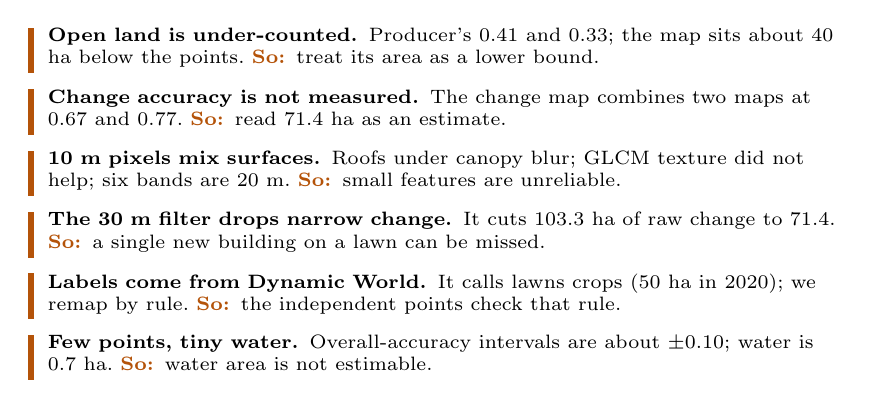
\begin{tikzpicture}
  \foreach \t/\b/\s [count=\i] in {
    Open land is under-counted/Producer's 0.41 and 0.33; the map sits about 40 ha below the points./treat its area as a lower bound,
    Change accuracy is not measured/The change map combines two maps at 0.67 and 0.77./read 71.4 ha as an estimate,
    10 m pixels mix surfaces/Roofs under canopy blur; GLCM texture did not help; six bands are 20 m./small features are unreliable,
    The 30 m filter drops narrow change/It cuts 103.3 ha of raw change to 71.4./a single new building on a lawn can be missed,
    Labels come from Dynamic World/It calls lawns crops (50 ha in 2020); we remap by rule./the independent points check that rule,
    Few points{,} tiny water/Overall-accuracy intervals are about $\pm$0.10; water is 0.7 ha./water area is not estimable}{
    \node[anchor=north west,text width=10.1cm,font=\scriptsize,inner sep=0,align=left] at (.25,-.78*\i+.78) {\textbf{\t.} \b\ {\color{saffron}\bfseries So:} \s.};
    \fill[saffron] (0,-.78*\i+.78) rectangle (.08,-.78*\i+.2);
  }
\end{tikzpicture}\\[3mm]
\capt{WHAT WE WOULD DO NEXT}\\[1.5mm]
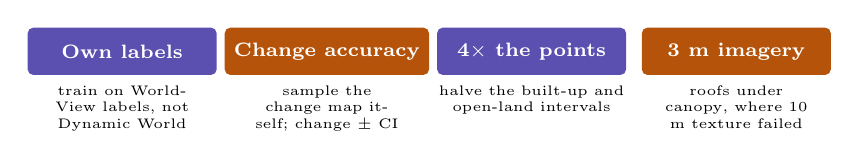
\begin{tikzpicture}
  \foreach \t/\d/\c [count=\i] in {Own labels/train on WorldView labels{,} not Dynamic World/iris,Change accuracy/sample the change map itself; change $\pm$ CI/saffron,4$\times$ the points/halve the built-up and open-land intervals/iris,3 m imagery/roofs under canopy{,} where 10 m texture failed/saffron}{
    \node[fill=\c,text=white,font=\scriptsize\bfseries,rounded corners=2pt,minimum width=2.4cm,minimum height=6mm,align=center] (c\i) at (2.6*\i-1.3,0) {\t};
    \node[anchor=north,text width=2.4cm,font=\tiny,align=center,inner sep=0] at ([yshift=-1.2mm]c\i.south) {\d};
  }
\end{tikzpicture}
\end{column}
\end{columns}
\end{frame}

% ---------------------------------------------------------------- team
\begin{frame}{Who did what}{TEAM}
% text pinned to the top; the three cards are drawn afterwards, as tall as the longest column
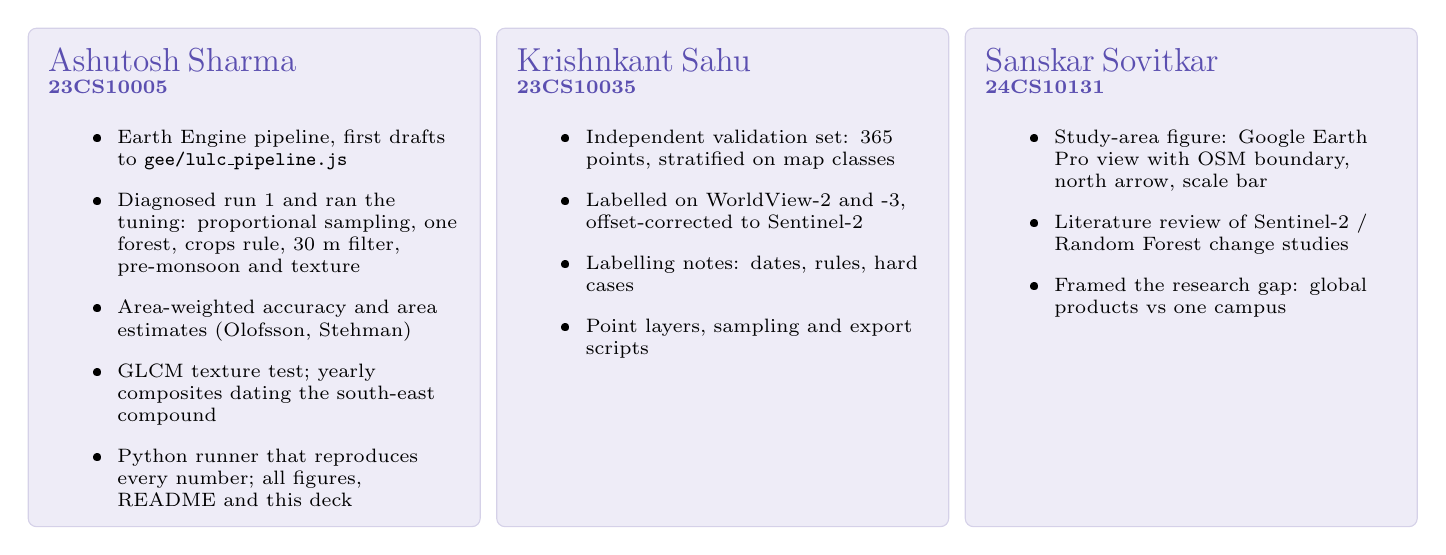
\begin{tikzpicture}[mem/.style={text width=5.25cm,inner sep=7pt,anchor=north west,font=\scriptsize,align=left}]
  \node[mem] (m1) at (0,0) {{\color{iris}\large Ashutosh Sharma}\\\capt{23CS10005}\\[2mm]
    \begin{itemize}\setlength\itemsep{1mm}
    \item Earth Engine pipeline, first drafts to \texttt{gee/lulc\_pipeline.js}
    \item Diagnosed run 1 and ran the tuning: proportional sampling, one forest, crops rule, 30 m filter, pre-monsoon and texture
    \item Area-weighted accuracy and area estimates (Olofsson, Stehman)
    \item GLCM texture test; yearly composites dating the south-east compound
    \item Python runner that reproduces every number; all figures, README and this deck
    \end{itemize}};
  \node[mem] (m2) at (5.95,0) {{\color{iris}\large Krishnkant Sahu}\\\capt{23CS10035}\\[2mm]
    \begin{itemize}\setlength\itemsep{1mm}
    \item Independent validation set: 365 points, stratified on map classes
    \item Labelled on WorldView-2 and -3, offset-corrected to Sentinel-2
    \item Labelling notes: dates, rules, hard cases
    \item Point layers, sampling and export scripts
    \end{itemize}};
  \node[mem] (m3) at (11.9,0) {{\color{iris}\large Sanskar Sovitkar}\\\capt{24CS10131}\\[2mm]
    \begin{itemize}\setlength\itemsep{1mm}
    \item Study-area figure: Google Earth Pro view with OSM boundary, north arrow, scale bar
    \item Literature review of Sentinel-2 / Random Forest change studies
    \item Framed the research gap: global products vs one campus
    \end{itemize}};
  \begin{pgfonlayer}{background}
    \path[card] let \p1=(m1.south), \p2=(m2.south), \p3=(m3.south), \n1={min(\y1,\y2,\y3)} in
      (0,0) rectangle (5.74,\n1) (5.95,0) rectangle (11.69,\n1) (11.9,0) rectangle (17.64,\n1);
  \end{pgfonlayer}
\end{tikzpicture}\\[3mm]

\begin{tikzpicture}
  \node[fill=ink,text=white,rounded corners=3pt,text width=17.2cm,inner sep=5pt,font=\scriptsize] {Code and results: \textbf{github.com/ashuwhy/landshift} \textperiodcentered\ gee/lulc\_pipeline.js \textperiodcentered\ scripts/run\_pipeline.py \textperiodcentered\ slides/make\_charts.py};
\end{tikzpicture}
\end{frame}

% ---------------------------------------------------------------- thanks
{\setbeamertemplate{footline}{}
\begin{frame}[plain]
\begin{tikzpicture}[remember picture,overlay]
  \fill[ink] (current page.north west) rectangle (current page.south east);
  \fill[gold] ([yshift=6mm]current page.south west) rectangle ([yshift=7.5mm]current page.south east);
  \node[anchor=east] at ([xshift=-6mm]current page.east) {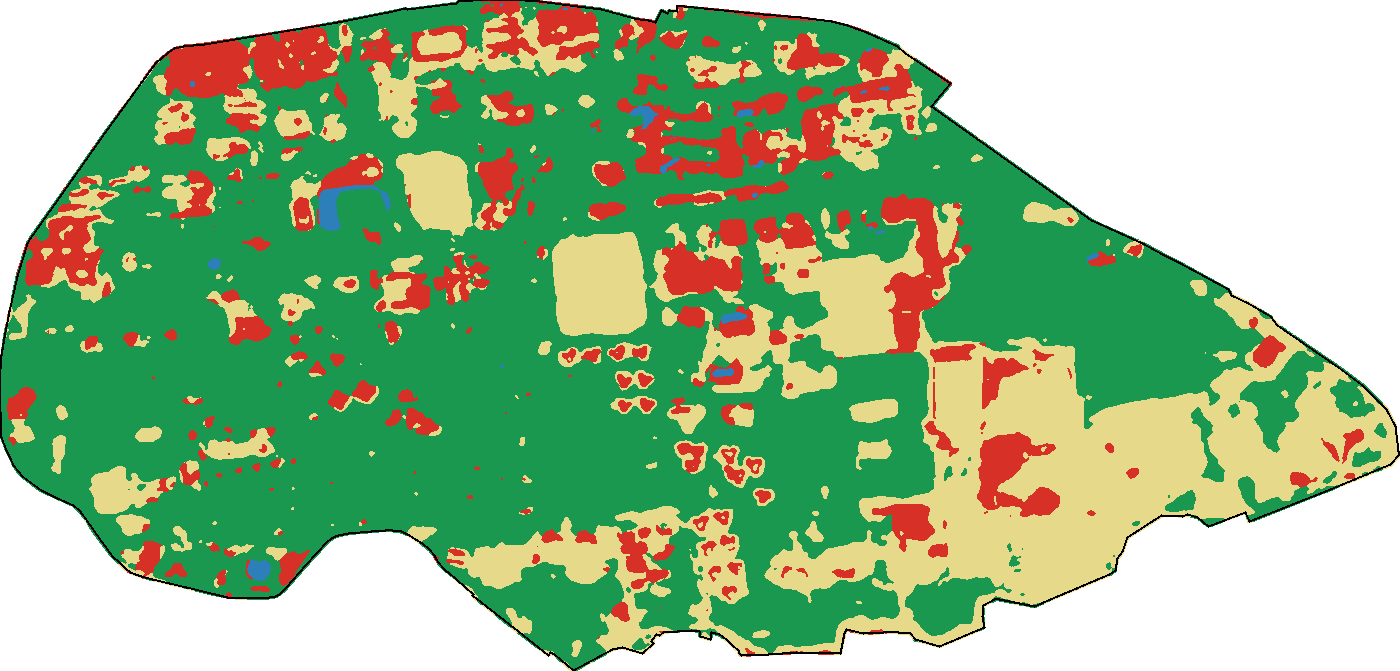
\includegraphics[width=10cm]{img/lulc_2025.png}};
  \node[anchor=north west,inner sep=0] at ([xshift=8mm,yshift=-8mm]current page.north west) {
\includegraphics[height=1.6cm]{img/iitkgp_logo_white}};
  \node[anchor=west,text=white,text width=6.6cm,align=left] at ([xshift=8mm,yshift=-3mm]current page.west) {%
    {\fontsize{30}{32}\selectfont\bfseries Thank you\par}\vspace{4mm}
    {\small 15.2\% of the campus changed,\\mostly open land turning green.\par}\vspace{4mm}
    {\color{gold}\scriptsize github.com/ashuwhy/landshift\par}\vspace{8mm}
    {\scriptsize Ashutosh Sharma\\Krishnkant Sahu\\Sanskar Sovitkar\par}};
\end{tikzpicture}
\end{frame}}

\end{document}
